% Options for packages loaded elsewhere
\PassOptionsToPackage{unicode}{hyperref}
\PassOptionsToPackage{hyphens}{url}
\documentclass[
  french,
  french,
  14pt,
  a4paper]{extarticle}
\usepackage{xcolor}
\usepackage[margin=2cm]{geometry}
\usepackage{amsmath,amssymb}
\setcounter{secnumdepth}{-\maxdimen} % remove section numbering
\usepackage{iftex}
\ifPDFTeX
  \usepackage[T1]{fontenc}
  \usepackage[utf8]{inputenc}
  \usepackage{textcomp} % provide euro and other symbols
\else % if luatex or xetex
  \usepackage{unicode-math} % this also loads fontspec
  \defaultfontfeatures{Scale=MatchLowercase}
  \defaultfontfeatures[\rmfamily]{Ligatures=TeX,Scale=1}
\fi
\usepackage{lmodern}
\ifPDFTeX\else
  % xetex/luatex font selection
  \setmainfont[]{Verdana}
\fi
% Use upquote if available, for straight quotes in verbatim environments
\IfFileExists{upquote.sty}{\usepackage{upquote}}{}
\IfFileExists{microtype.sty}{% use microtype if available
  \usepackage[]{microtype}
  \UseMicrotypeSet[protrusion]{basicmath} % disable protrusion for tt fonts
}{}
\makeatletter
\@ifundefined{KOMAClassName}{% if non-KOMA class
  \IfFileExists{parskip.sty}{%
    \usepackage{parskip}
  }{% else
    \setlength{\parindent}{0pt}
    \setlength{\parskip}{6pt plus 2pt minus 1pt}}
}{% if KOMA class
  \KOMAoptions{parskip=half}}
\makeatother
\usepackage{longtable,booktabs,array}
\newcounter{none} % for unnumbered tables
\usepackage{calc} % for calculating minipage widths
% Correct order of tables after \paragraph or \subparagraph
\usepackage{etoolbox}
\makeatletter
\patchcmd\longtable{\par}{\if@noskipsec\mbox{}\fi\par}{}{}
\makeatother
% Allow footnotes in longtable head/foot
\IfFileExists{footnotehyper.sty}{\usepackage{footnotehyper}}{\usepackage{footnote}}
\makesavenoteenv{longtable}
\ifLuaTeX
\usepackage[bidi=basic,shorthands=off]{babel}
\else
\usepackage[bidi=default,shorthands=off]{babel}
\fi
\ifPDFTeX
\else
\babelfont{rm}[]{Verdana}
\fi
\ifLuaTeX
  \usepackage{selnolig} % disable illegal ligatures
\fi
\setlength{\emergencystretch}{3em} % prevent overfull lines
\providecommand{\tightlist}{%
  \setlength{\itemsep}{0pt}\setlength{\parskip}{0pt}}
\usepackage{wrapfig}
\usepackage{tabularx}
\usepackage{graphicx}
\usepackage{xcolor}
\setlength{\parskip}{1.2em}

% Child-friendly line breaking: left-aligned (never justified) so that words
% are NEVER split across two lines with a hyphen — easier for a young reader.
% Done with built-in primitives (no extra package needed).
\hyphenpenalty=10000
\exhyphenpenalty=10000
\tolerance=9999
% Soft ragged-right: lines fill the column but may stop up to 2em short of the
% margin. Plain \raggedright (infinite stretch) made lines break far too early
% in the narrow column beside a wrapfig image (short, one-word first lines).
% Word-splitting stays OFF via the hyphenpenalties above, not via the margin.
\AtBeginDocument{\rightskip=0pt plus 2em\relax\parindent=0pt}

\definecolor{accentcolor}{RGB}{40, 80, 140}

% Big, decorated divider title for the 4 section opener pages.
% Usage: \sectiondivider{1}{Textes courts}
\newcommand{\sectiondivider}[2]{%
  \vspace*{2cm}%
  \begin{center}
    {\fontsize{18pt}{22pt}\selectfont\textcolor{accentcolor}{\MakeUppercase{Section #1}}}\\[0.6em]
    \textcolor{accentcolor}{\rule{0.35\textwidth}{1.5pt}}\\[1em]
    {\fontsize{38pt}{44pt}\selectfont\bfseries #2}
  \end{center}
  \vspace{1.5cm}
}

% Per-chapter body font, used by fit_pages.py to fit each chapter on exactly
% one page. Usage (wrapped around a whole chapter): {\storyfont{12} ... }
% baseline = 1.2 x size, parskip scaled down to save vertical space.
\newcommand{\storyfont}[1]{%
  \setlength{\parskip}{0.6em}%
  \fontsize{#1pt}{\dimexpr #1pt*6/5\relax}\selectfont%
}
\usepackage{bookmark}
\IfFileExists{xurl.sty}{\usepackage{xurl}}{} % add URL line breaks if available
\urlstyle{same}
\hypersetup{
  pdftitle={Une année avec Mango},
  pdflang={fr-FR},
  hidelinks,
  pdfcreator={LaTeX via pandoc}}

\title{Une année avec Mango}
\usepackage{etoolbox}
\makeatletter
\providecommand{\subtitle}[1]{% add subtitle to \maketitle
  \apptocmd{\@title}{\par {\large #1 \par}}{}{}
}
\makeatother
\subtitle{Livret de Lecture - Fluence CE1}
\author{}
\date{}

\begin{document}
\maketitle

\begin{center}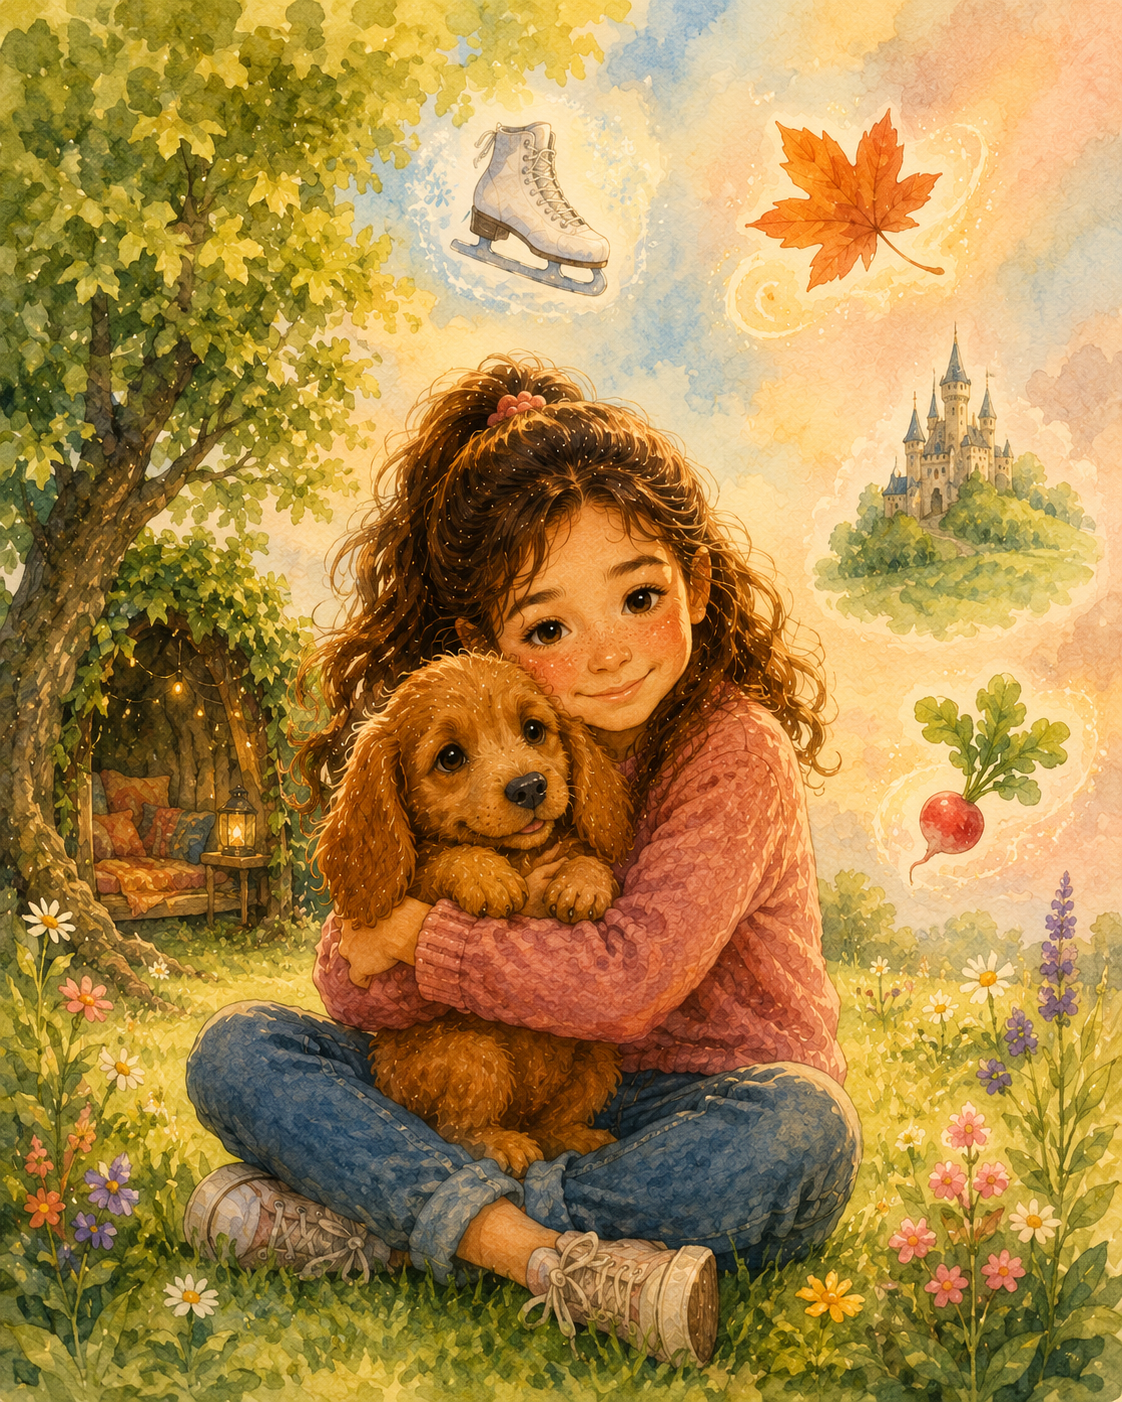
\includegraphics[width=0.75\linewidth]{img/cover_v2.png}\end{center}

\begin{center}\textit{Yaëlle et Camille Chaudy, 2026}\end{center}

\section{Une année avec Mango}\label{une-annuxe9e-avec-mango}

\subsection{Comment utiliser ce
livret}\label{comment-utiliser-ce-livret}

Ce livret raconte l'histoire de Camille et de son chien Mango, en \textbf{16 chapitres}. On les lit dans l'ordre, comme un petit roman.

Les chapitres deviennent peu à peu \textbf{plus longs et plus riches}, divisés en \textbf{4 sections} de difficulté croissante :

\begin{itemize}
\tightlist
\item
  \textbf{Section 1 - Chapitres courts} : phrases très simples, pour
  démarrer en confiance (\textasciitilde180 mots, 2 min de lecture)
\item
  \textbf{Section 2 - Niveau 1} : phrases courtes, mots simples
  (\textasciitilde270 mots, 3 min de lecture)
\item
  \textbf{Section 3 - Niveau 2} : un peu plus riches
  (\textasciitilde360 mots, 4 min de lecture)
\item
  \textbf{Section 4 - Niveau 3} : niveau CE1 complet
  (\textasciitilde450 mots, 5 min de lecture)
\end{itemize}

L'histoire est \textbf{originale}, elle peut être imprimée, copiée ou modifiée librement.

\subsubsection{Conseils pour l'adulte}\label{conseils-pour-ladulte}

\begin{enumerate}
\def\labelenumi{\arabic{enumi}.}
\tightlist
\item
  \textbf{Lire ensemble une première fois}, sans chronomètre. L'enfant écoute, puis répète.
\item
  \textbf{Lire seul.e une deuxième fois}, en se chronométrant. Noter le temps et les erreurs dans le tableau de suivi.
\item
  \textbf{Discuter du chapitre} avec les questions de compréhension. Lire, ce n'est pas seulement déchiffrer : c'est aussi comprendre.
\item
  \textbf{Refaire le même chapitre} plusieurs fois. La vitesse augmente, c'est très motivant ! On passe au chapitre suivant une fois le niveau de lecture atteint.
\end{enumerate}

\begin{quote}
\textbf{Objectif de fin de CE1} : lire environ 90 mots par minute.
\end{quote}

\begin{center}\rule{0.5\linewidth}{0.5pt}\end{center}

\newpage

\sectiondivider{1}{Chapitres courts}

\subsubsection{Pour bien commencer}\label{pour-bien-commencer}

Les chapitres de cette section sont \textbf{très courts} (environ
\textbf{180 mots}). Les phrases sont courtes (moins de 10 mots). Le
vocabulaire est simple et tout est au \textbf{présent}.

C'est un bon endroit pour démarrer, prendre confiance et trouver son
rythme. C'est aussi le début de l'histoire : on fait la connaissance de
Camille, de sa famille et de ses rêves.

\subsubsection{Combien de temps pour lire un chapitre
?}\label{combien-de-temps-pour-lire-un-chapitre}

{\def\LTcaptype{none} % do not increment counter
\begin{longtable}[]{@{}lll@{}}
\toprule\noalign{}
Niveau de référence & Vitesse & Temps pour \textasciitilde180 mots \\
\midrule\noalign{}
\endhead
\bottomrule\noalign{}
\endlastfoot
Fin de CP & 50 mots/min & \textasciitilde3 min 35 s \\
Fin de CE1 & 90 mots/min & \textbf{\textasciitilde{} 2 min} \\
Fin de CE2 & 110 mots/min & \textasciitilde1 min 40 s \\
\end{longtable}
}

\begin{quote}
\emph{Petit conseil :} compare-toi à toi-même, pas à ces chiffres. Ton
meilleur temps, c'est celui que tu améliores la fois d'après !
\end{quote}

\newpage
% <<FIT 1>>
{\storyfont{12}%

\section{Chapitre 1 --- Moi, c'est
Camille}\label{chapitre-1-moi-cest-camille}

\begin{wrapfigure}{r}{7cm}
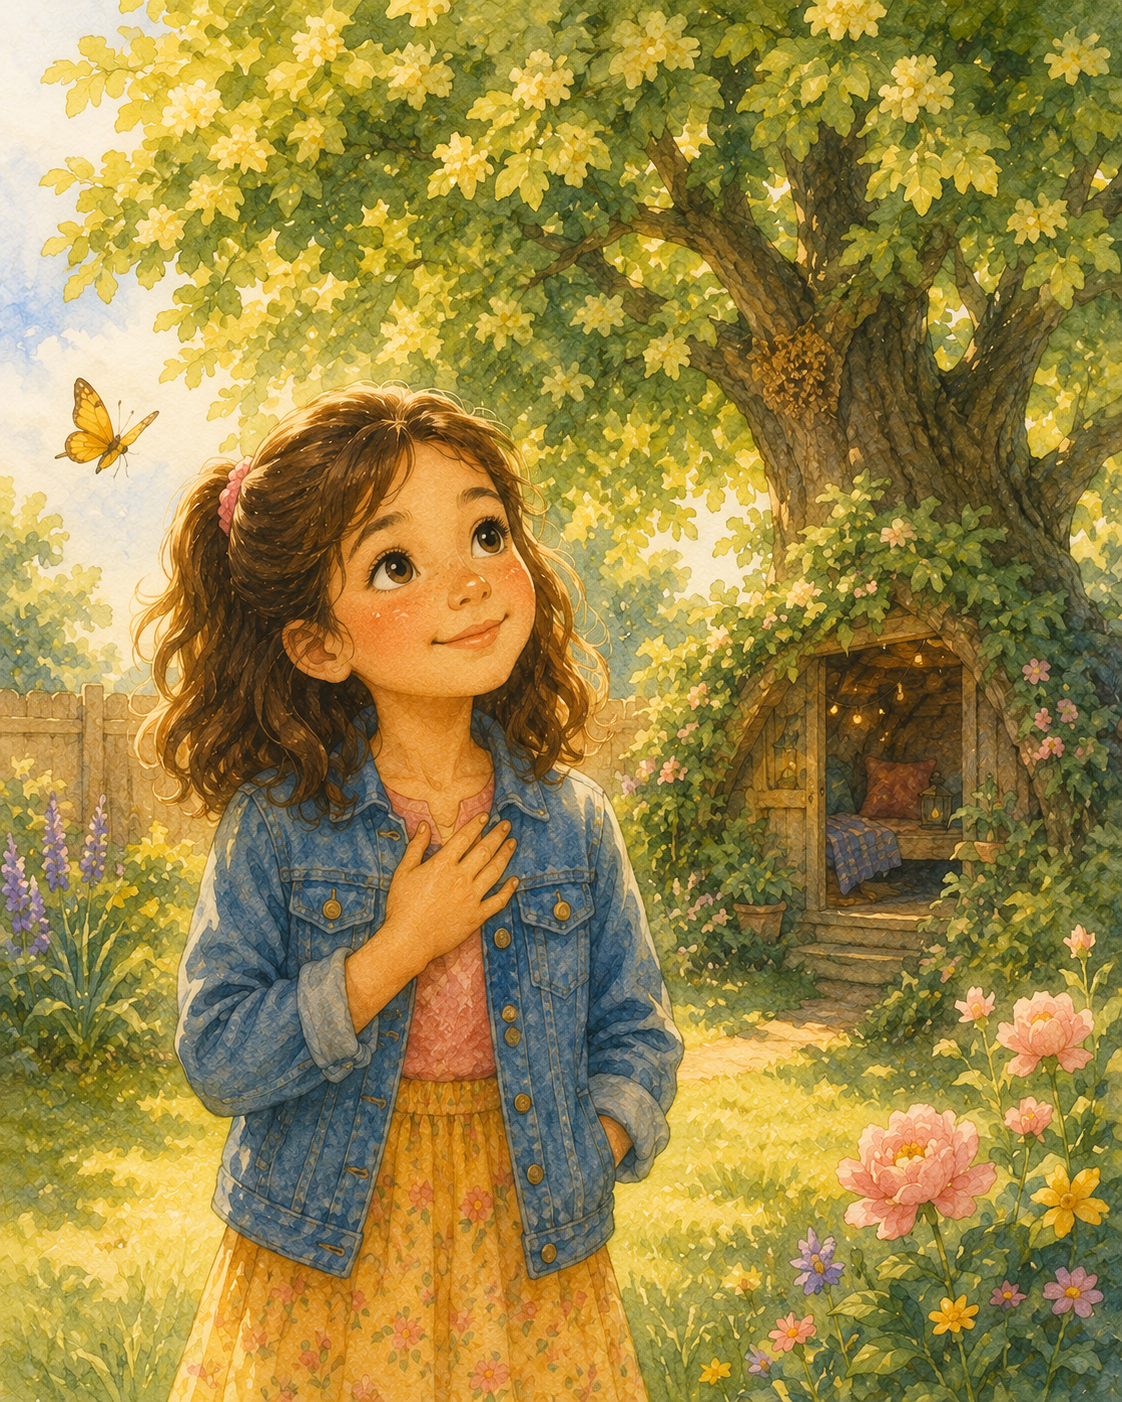
\includegraphics[width=7cm]{img/ch01_camille.png}
\end{wrapfigure}

Bonjour ! Moi, c'est Camille. J'ai huit ans. J'habite une petite maison
avec un grand jardin.

Dans ma famille, nous sommes cinq. Il y a papa, maman, et mes deux
sœurs. Ma grande sœur s'appelle Émilie. Elle a dix ans. Ma petite sœur
s'appelle Lina. Elle a six ans.

Émilie est grande et gentille. Elle sait faire du patin à glace. Lina
est petite et rigolote. Elle pose mille questions par jour.

Moi, j'adore le jardin. Il y a des fleurs, un vieux tilleul et beaucoup
d'herbe. Au fond, il y a une cabane. C'est mon endroit préféré.

J'aime aussi les animaux. J'aime les chiens. J'aime les chats. J'aime
les oiseaux du jardin.

Mais il manque quelque chose à la maison. Nous n'avons pas d'animal. Pas
encore\ldots{}

Le soir, je regarde par la fenêtre. Je rêve d'un petit chien à moi. Un
chien qui court dans le jardin. Un chien qui dort près de mon lit.

Un jour, peut-être, mon rêve va se réaliser.

Voici mon histoire. Elle commence au printemps.

\begin{center}\rule{0.5\linewidth}{0.5pt}\end{center}

\subsubsection{Questions de
compréhension}\label{questions-de-compruxe9hension}

\begin{enumerate}
\def\labelenumi{\arabic{enumi}.}
\tightlist
\item
  Comment s'appellent les deux sœurs de Camille ?
\item
  Quel est l'endroit préféré de Camille dans le jardin ?
\item
  De quoi rêve Camille, le soir ?
\end{enumerate}

\subsubsection{Mon suivi de lecture}\label{mon-suivi-de-lecture}

\begin{center}
\begin{tabularx}{\textwidth}{|X|X|}
\hline
\textbf{Date} & \textbf{Temps} \\
\hline
& \\
\hline
& \\
\hline
& \\
\hline
& \\
\hline
& \\
\hline
\end{tabularx}
\end{center}

}% <<FIT END 1>>
\newpage
% <<FIT 2>>
{\storyfont{13}%

\section{Chapitre 2 --- Ma meilleure amie
Suzanne}\label{chapitre-2-ma-meilleure-amie-suzanne}

\begin{wrapfigure}{r}{7cm}
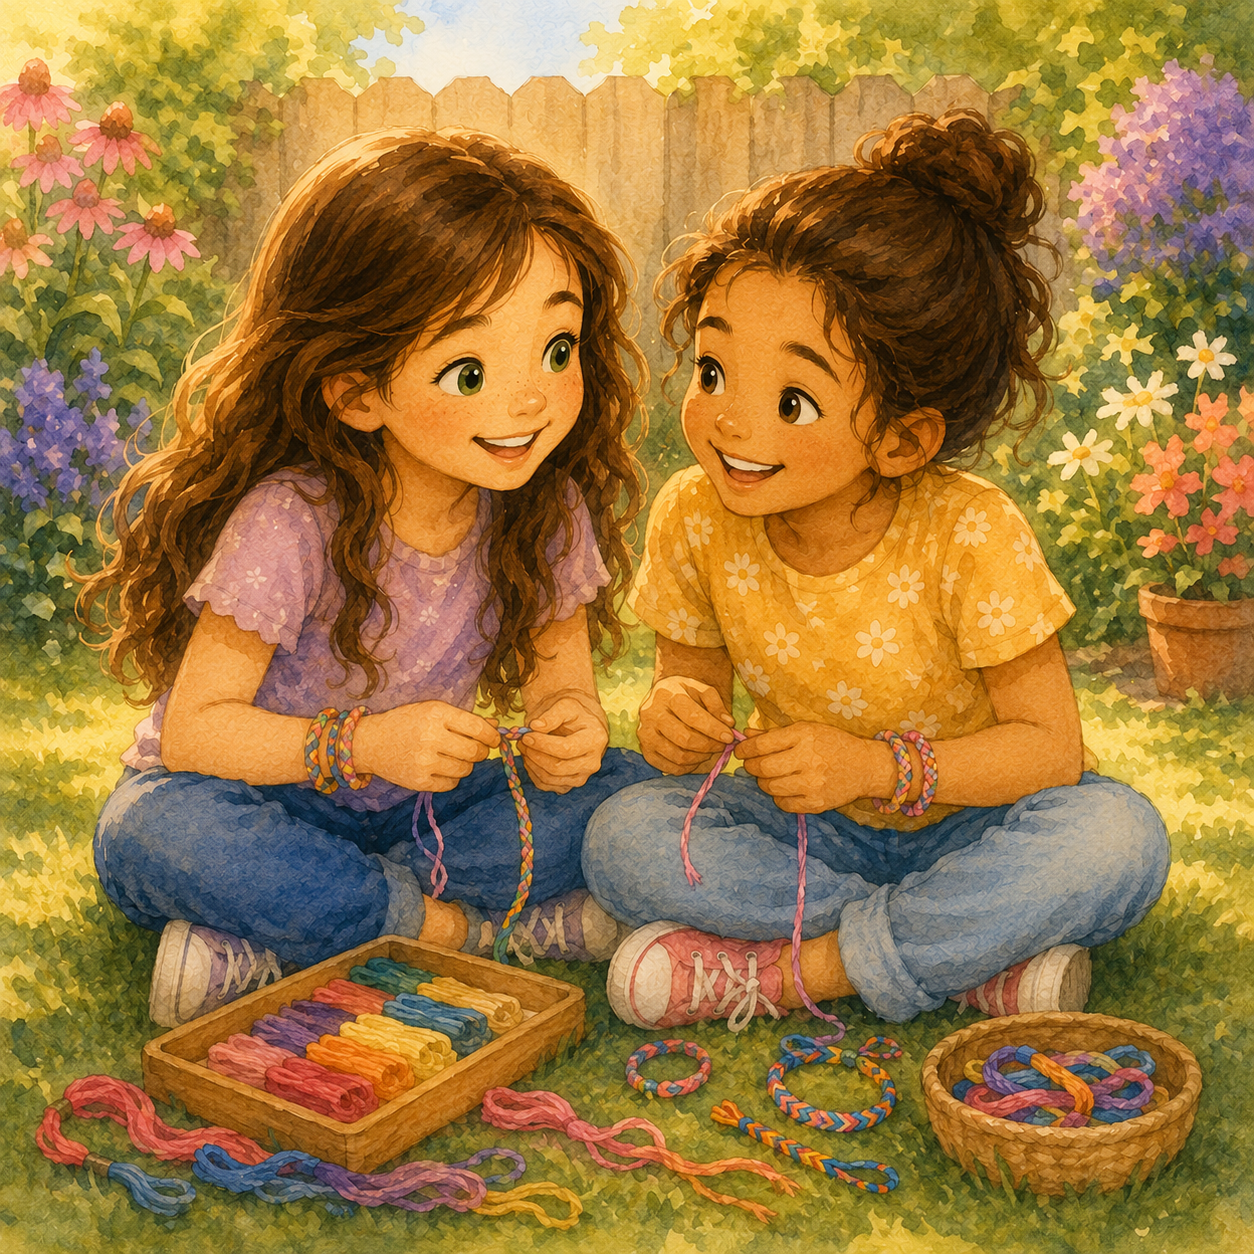
\includegraphics[width=7cm]{img/amie.png}
\end{wrapfigure}

Ma meilleure amie s'appelle Suzanne. Elle a huit ans, comme moi. Nous
sommes dans la même classe.

Suzanne a de longs cheveux bruns. Elle a des yeux verts. Elle rit tout
le temps. Son rire est très joyeux.

À la récré, on est toujours ensemble. On adore la corde à sauter. On
adore le dessin. Parfois, on chante des chansons rigolotes.

Suzanne habite tout près de chez moi. Le mercredi, je vais chez elle. On
fait des bracelets. On joue dans le jardin. Sa maman fait un bon goûter.

Quand je suis triste, Suzanne me console. Elle me dit des mots tout
doux. Et quand elle est triste, je fais pareil. C'est ça, une vraie
amie.

Suzanne aime beaucoup les animaux, comme moi. Elle a un poisson rouge.
Il s'appelle Bulle.

Suzanne connaît mon grand rêve. Je veux un petit chien. Suzanne trouve
que c'est une super idée.

« Si tu as un chien, dit-elle, je joue avec lui tous les mercredis ! »

Vivement le prochain mercredi.

\begin{center}\rule{0.5\linewidth}{0.5pt}\end{center}

\subsubsection{Questions de
compréhension}\label{questions-de-compruxe9hension-1}

\begin{enumerate}
\def\labelenumi{\arabic{enumi}.}
\tightlist
\item
  Quel âge a Suzanne ?
\item
  Que font les deux amies à la récré ?
\item
  Quel animal a Suzanne à la maison ?
\end{enumerate}

\subsubsection{Mon suivi de lecture}\label{mon-suivi-de-lecture-1}

\begin{center}
\begin{tabularx}{\textwidth}{|X|X|}
\hline
\textbf{Date} & \textbf{Temps} \\
\hline
& \\
\hline
& \\
\hline
& \\
\hline
\end{tabularx}
\end{center}

}% <<FIT END 2>>
\newpage
% <<FIT 3>>
{\storyfont{13}%

\section{Chapitre 3 --- Ma cabane
secrète}\label{chapitre-3-ma-cabane-secruxe8te}

\begin{wrapfigure}{r}{7cm}

\includegraphics[width=7cm]{img/ch03_cabane.png}
\end{wrapfigure}

Au fond du jardin, il y a un grand arbre. Sous ses branches, on ne voit
rien du dehors. C'est mon endroit préféré au monde.

C'est ma cabane secrète. Personne ne la connaît. Pas même ma petite sœur
Lina.

Pour entrer, j'écarte deux branches. C'est comme un rideau. À
l'intérieur, tout est vert et doux. Le sol est couvert de feuilles.
Au-dessus, je vois le ciel.

Sur le sol, il y a un coussin rouge. À côté, il y a une petite boîte en
bois. Dedans, je cache mes trésors.

Dans ma boîte, j'ai un caillou brillant. J'ai une plume bleue. J'ai un
coquillage. Et j'ai un petit dessin de Suzanne.

Quand je suis dans ma cabane, je rêve très fort. Je deviens une pirate.
Je deviens une exploratrice. Parfois, je suis même une fée.

Souvent, je pense à mon rêve de chien. J'imagine un petit chien, ici,
avec moi.

Quand je suis triste ou fâchée, je viens ici. Et tout de suite, je me
sens mieux.

Cette cabane, c'est mon petit royaume à moi.

\begin{center}\rule{0.5\linewidth}{0.5pt}\end{center}

\subsubsection{Questions de
compréhension}\label{questions-de-compruxe9hension-2}

\begin{enumerate}
\def\labelenumi{\arabic{enumi}.}
\tightlist
\item
  Où se trouve la cabane secrète ?
\item
  Qu'est-ce que Camille cache dans sa petite boîte ?
\item
  Qui connait la cabane secrète ?
\end{enumerate}

\subsubsection{Mon suivi de lecture}\label{mon-suivi-de-lecture-2}

\begin{center}
\begin{tabularx}{\textwidth}{|X|X|}
\hline
\textbf{Date} & \textbf{Temps} \\
\hline
& \\
\hline
& \\
\hline
& \\
\hline
\end{tabularx}
\end{center}

}% <<FIT END 3>>
\newpage
% <<FIT 4>>
{\storyfont{12}%

\section{Chapitre 4 --- Une grande
nouvelle}\label{chapitre-4-une-grande-nouvelle}

\begin{wrapfigure}{r}{7cm}
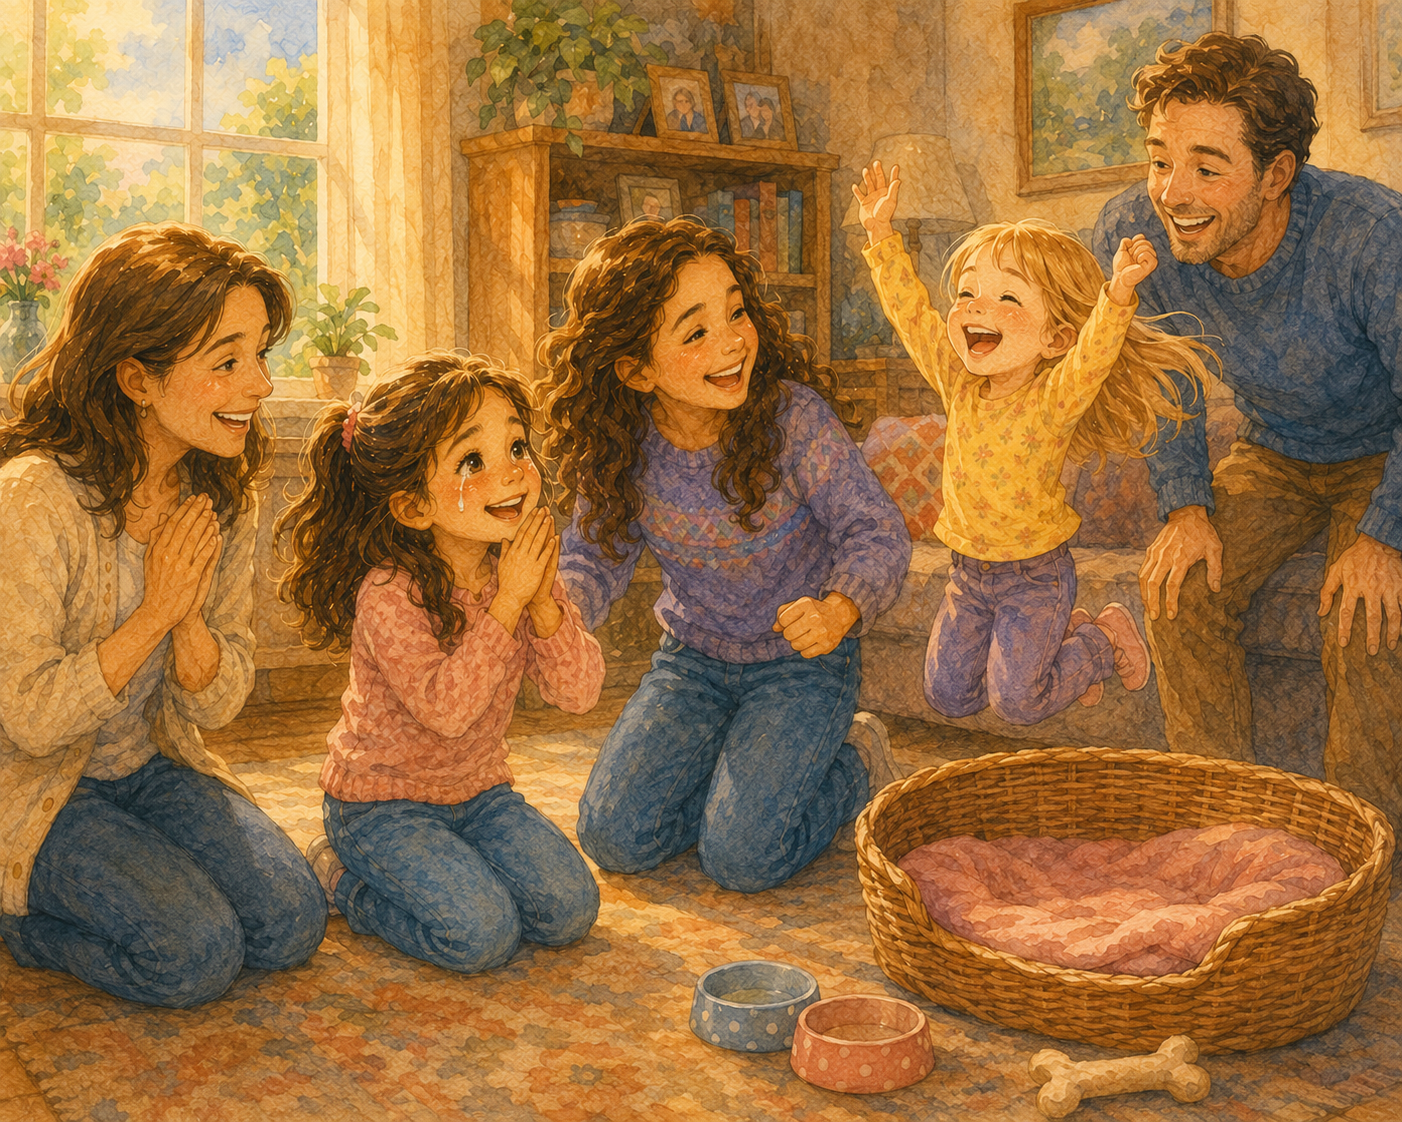
\includegraphics[width=7cm]{img/ch04_nouvelle.png}
\end{wrapfigure}

Ce matin, papa a un grand sourire. Maman aussi. Je sens qu'il se passe
quelque chose.

« Les filles, dit papa, nous avons une nouvelle pour vous. »

Émilie, Lina et moi, on écoute bien. Mon cœur bat vite.

« Bientôt, dit maman, un petit chien va venir vivre avec nous. »

Je n'en crois pas mes oreilles. Un chien ! Un vrai chien à nous !

Lina saute partout. Émilie rit. Moi, j'ai les larmes aux yeux. C'est mon
rêve qui se réalise.

« C'est un bébé chien, dit papa. Il a deux mois. Il est tout brun. »

On cherche tous un nom. Lina veut l'appeler « Bonbon ». Émilie préfère «
Caramel ».

Moi, je pense à sa belle couleur brune, comme un fruit doré.

« Et si on l'appelait Mango ? » je propose.

Tout le monde adore ce nom. Mango ! C'est décidé.

Maintenant, on prépare la maison. On installe un panier. On achète des
gamelles et un petit jouet.

Demain, Mango arrive. Je suis trop contente. Je crois que je ne vais pas
dormir !

\begin{center}\rule{0.5\linewidth}{0.5pt}\end{center}

\subsubsection{Questions de
compréhension}\label{questions-de-compruxe9hension-3}

\begin{enumerate}
\def\labelenumi{\arabic{enumi}.}
\tightlist
\item
  Quelle est la grande nouvelle annoncée par les parents ?
\item
  Qui propose le nom de Mango, et pourquoi ce nom ?
\item
  Que fait la famille pour préparer la maison ?
\end{enumerate}

\subsubsection{Mon suivi de lecture}\label{mon-suivi-de-lecture-3}

\begin{center}
\begin{tabularx}{\textwidth}{|X|X|}
\hline
\textbf{Date} & \textbf{Temps} \\
\hline
& \\
\hline
& \\
\hline
& \\
\hline
\end{tabularx}
\end{center}

}% <<FIT END 4>>
\newpage

\sectiondivider{2}{Niveau 1}

\subsubsection{On progresse !}\label{on-progresse}

Les chapitres de cette section sont un peu plus longs (environ
\textbf{270 mots}). Les phrases restent courtes, le vocabulaire reste
simple, et tout est presque toujours au \textbf{présent}.

Dans cette partie de l'histoire, Mango arrive enfin à la maison. La vie
de Camille change pour de bon !

\subsubsection{Combien de temps pour lire un chapitre
?}\label{combien-de-temps-pour-lire-un-chapitre-1}

{\def\LTcaptype{none} % do not increment counter
\begin{longtable}[]{@{}lll@{}}
\toprule\noalign{}
Niveau de référence & Vitesse & Temps pour \textasciitilde270 mots \\
\midrule\noalign{}
\endhead
\bottomrule\noalign{}
\endlastfoot
Fin de CP & 50 mots/min & \textasciitilde5 min 25 s \\
Fin de CE1 & 90 mots/min & \textbf{\textasciitilde{} 3 min} \\
Fin de CE2 & 110 mots/min & \textasciitilde2 min 30 s \\
\end{longtable}
}

\newpage
% <<FIT 5>>
{\storyfont{12}%

\section{Chapitre 5 --- Le premier jour de
Mango}\label{chapitre-5-le-premier-jour-de-mango}

\begin{wrapfigure}{r}{7cm}
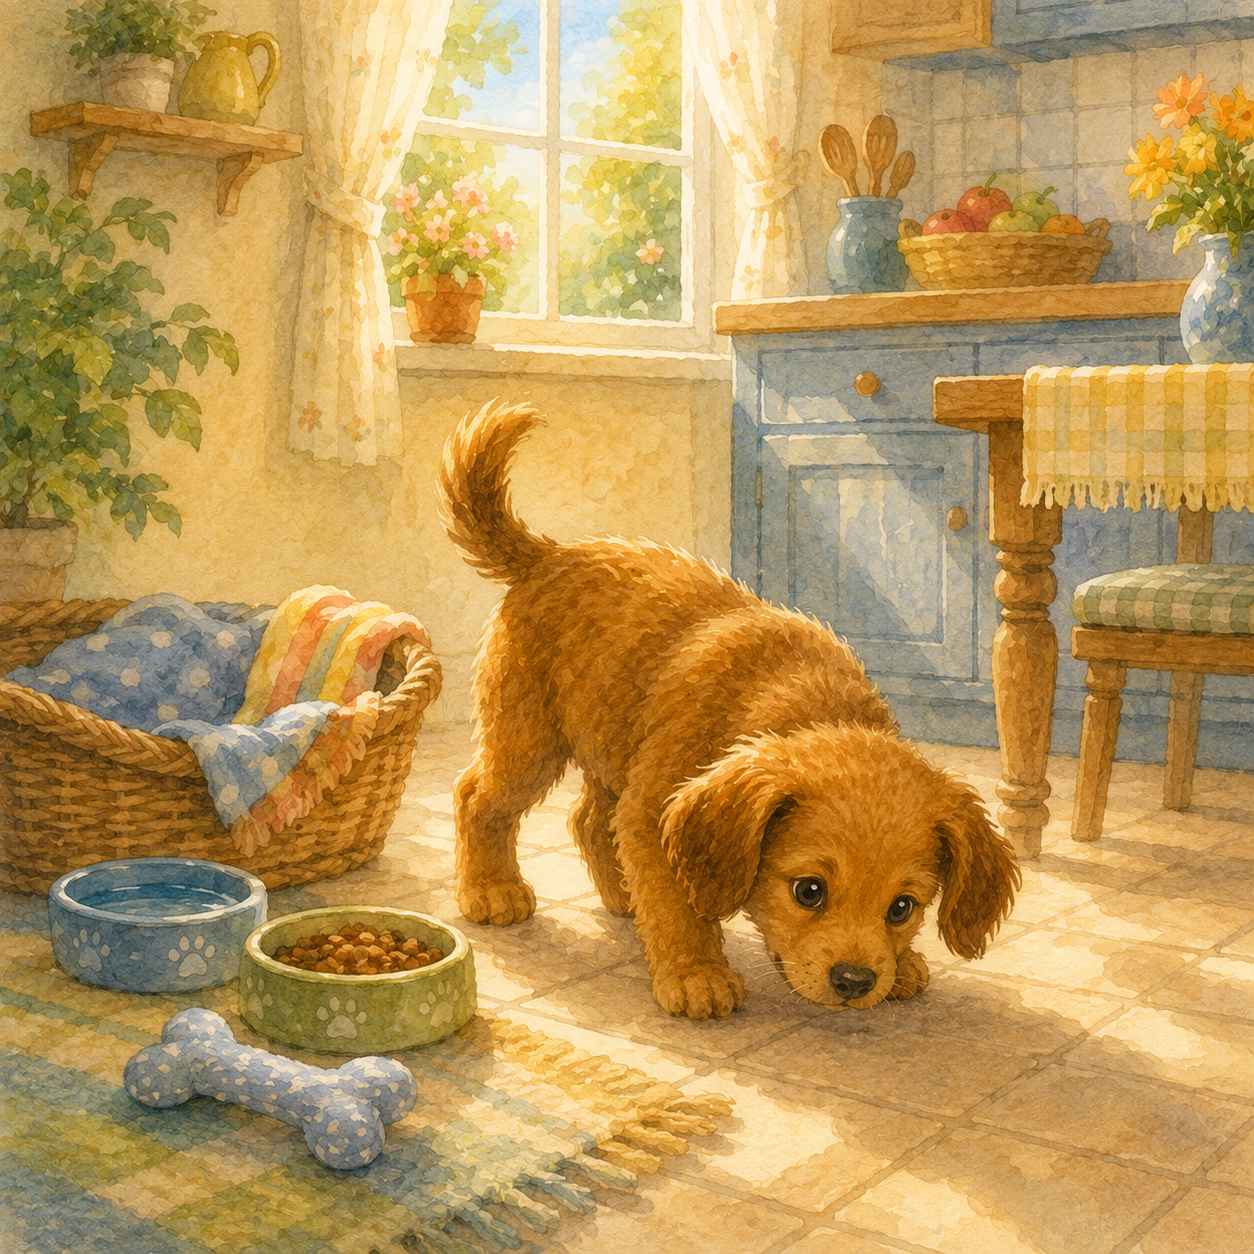
\includegraphics[width=7cm]{img/mango.png}
\end{wrapfigure}

C'est le grand jour. Mango arrive à la maison.

Quand papa pose Mango sur le sol, le petit chien tremble un peu. Il a
deux mois. Il est tout brun, avec de grandes oreilles tombantes. Sa
queue ne s'arrête jamais de bouger.

Mango regarde partout. Tout est nouveau pour lui : la maison, les
bruits, les odeurs, et nous. Je m'approche tout doucement. Je tends ma
main. Mango sent mes doigts avec son petit nez froid. Puis il me lèche
la main. Je crois qu'il m'aime déjà !

Lina veut le caresser tout de suite. « Doucement », dit maman. « Il a un
peu peur. » Lina caresse Mango avec un seul doigt. Émilie, elle, reste
calme et le laisse venir vers elle.

Maman a tout préparé. Dans un coin de la cuisine, il y a un panier avec
une couverture douce. À côté, il y a deux gamelles. Une pour l'eau, une
pour les croquettes. Et il y a un petit jouet en forme d'os.

Mango va voir son panier. Il monte dedans et se couche en boule. Mais
cinq minutes plus tard, il en sort. Il veut tout découvrir. Il sent
chaque coin, chaque meuble. Il met même son nez dans mes chaussures !

À midi, Mango mange pour la première fois. Il avale ses croquettes très
vite. Ensuite, il boit beaucoup d'eau.

Le soir, Mango est fatigué. Il s'endort dans son panier. Je le regarde
dormir. Maintenant, j'ai un ami à quatre pattes. Et c'est le plus beau
jour de ma vie.

\begin{center}\rule{0.5\linewidth}{0.5pt}\end{center}

\subsubsection{Questions de
compréhension}\label{questions-de-compruxe9hension-4}

\begin{enumerate}
\def\labelenumi{\arabic{enumi}.}
\tightlist
\item
  Quel âge a Mango, et de quelle couleur est-il ?
\item
  Comment Lina caresse-t-elle Mango la première fois ?
\item
  Qu'est-ce que maman a préparé pour lui dans la cuisine ?
\end{enumerate}

\subsubsection{Mon suivi de lecture}\label{mon-suivi-de-lecture-4}

\begin{center}
\begin{tabularx}{\textwidth}{|X|X|}
\hline
\textbf{Date} & \textbf{Temps} \\
\hline
& \\
\hline
& \\
\hline
& \\
\hline
\end{tabularx}
\end{center}

}% <<FIT END 5>>
\newpage
% <<FIT 6>>
{\storyfont{12}%

\section{Chapitre 6 --- La cabane et le
trésor}\label{chapitre-6-la-cabane-et-le-truxe9sor}

\begin{wrapfigure}{r}{7cm}
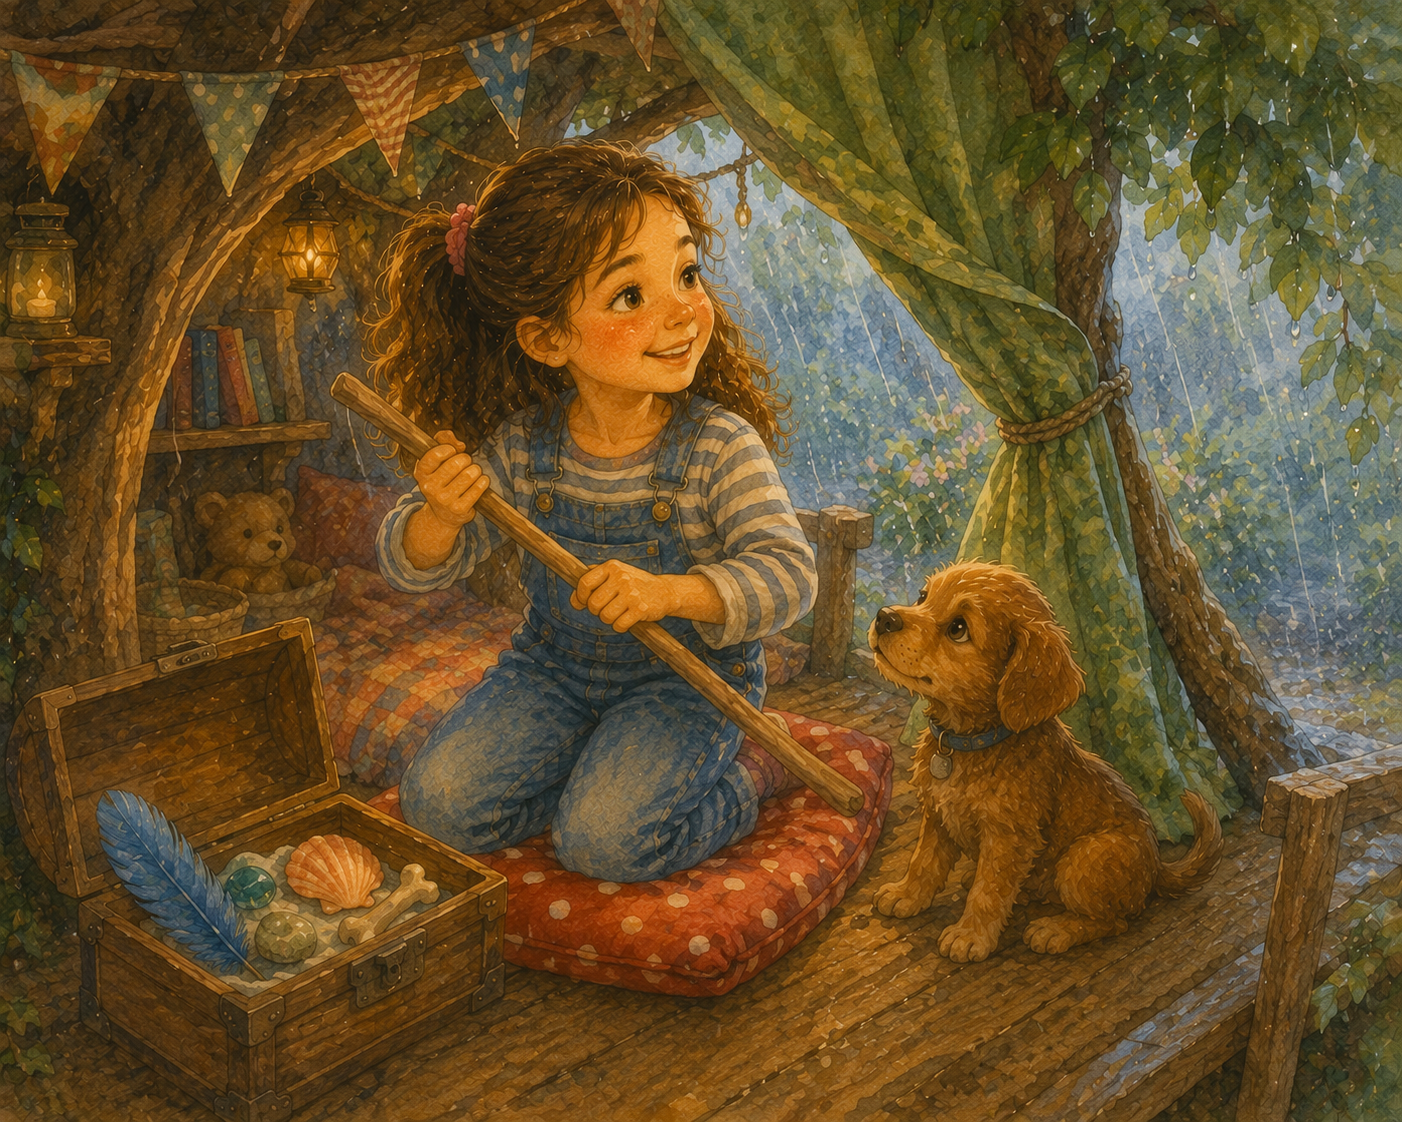
\includegraphics[width=7cm]{img/ch06_tresor.png}
\end{wrapfigure}

Aujourd'hui, il pleut. Je ne peux pas jouer dehors longtemps. Alors
j'emmène Mango dans ma cabane secrète, au fond du jardin.

C'est la première fois que Mango entre dans la cabane. Il sent partout
avec son petit nez. Il regarde le coussin rouge. Il regarde ma boîte à
trésors. Tout est nouveau pour lui.

« Bienvenue dans mon royaume », je lui dis tout bas. Mango remue la
queue. Je crois qu'il aime déjà cet endroit.

Sous les branches, on entend la pluie qui tombe. Ça fait un bruit tout
doux : « ploc, ploc, ploc ». Dans la cabane, on est bien au sec et bien
au chaud.

Aujourd'hui, je décide qu'on part à l'aventure. La cabane devient un
grand bateau. Moi, je suis le capitaine. Mango, lui, est mon matelot.
Dehors, ce n'est plus le jardin : c'est la mer ! La pluie, ce sont les
vagues.

« En avant, Mango ! » Je tiens un bâton comme une rame. Mango aboie,
comme s'il comprenait tout. On cherche une île au trésor.

Soudain, je « trouve » le trésor : c'est ma boîte en bois ! Je l'ouvre.
Dedans, il y a mon caillou brillant, ma plume bleue et mon coquillage.
Pour Mango, j'ajoute un nouveau trésor : un de ses petits os en
plastique.

Quand la pluie s'arrête, on rentre à la maison. On est un peu fatigués,
mais très contents.

Maintenant, Mango connaît mon secret. Et tu sais quoi ? Je crois que la
cabane lui plaît autant qu'à moi. Demain, on repart à l'aventure !

\begin{center}\rule{0.5\linewidth}{0.5pt}\end{center}

\subsubsection{Questions de
compréhension}\label{questions-de-compruxe9hension-5}

\begin{enumerate}
\def\labelenumi{\arabic{enumi}.}
\tightlist
\item
  Pourquoi Camille emmène-t-elle Mango dans la cabane, aujourd'hui ?
\item
  En quoi se transforme la cabane pendant l'aventure ?
\item
  Quel nouveau trésor Camille ajoute-t-elle dans sa boîte ?
\end{enumerate}

\subsubsection{Mon suivi de lecture}\label{mon-suivi-de-lecture-5}

\begin{center}
\begin{tabularx}{\textwidth}{|X|X|}
\hline
\textbf{Date} & \textbf{Temps} \\
\hline
& \\
\hline
& \\
\hline
& \\
\hline
\end{tabularx}
\end{center}

}% <<FIT END 6>>
\newpage
% <<FIT 7>>
{\storyfont{12}%

\section{Chapitre 7 --- On plante un
jardin}\label{chapitre-7-on-plante-un-jardin}

\begin{wrapfigure}{r}{7cm}
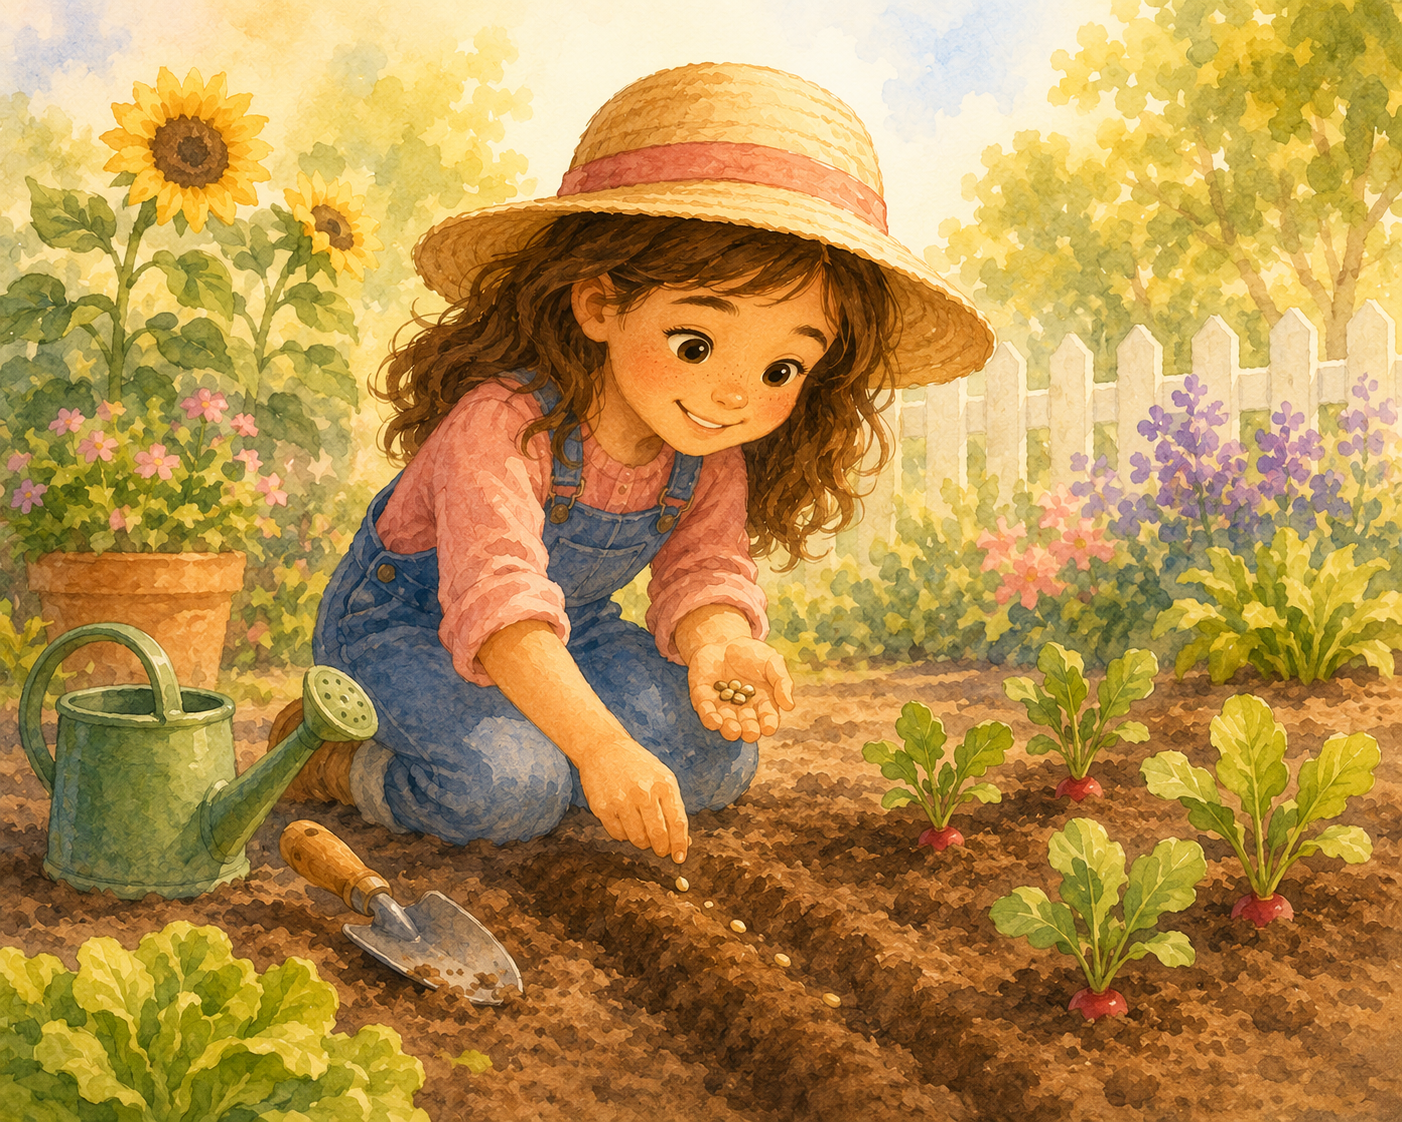
\includegraphics[width=7cm]{img/radis.png}
\end{wrapfigure}

Au printemps, maman a une idée. « Et si vous plantiez un petit jardin ?
» Émilie, Lina et moi, on dit oui tout de suite. Suzanne vient nous
aider, comme chaque mercredi.

Maman nous donne un sachet de graines de radis. Les radis sont faciles à
faire pousser. On choisit un coin de jardin, bien au soleil. Les radis
aiment la lumière.

Avec une petite pelle, je fais une ligne. Lina met des graines sur la
ligne, bien espacées. Suzanne recouvre les graines avec un peu de terre.
Émilie tape doucement avec sa main. Puis on arrose tout avec l'arrosoir.

Pendant ce temps, Mango nous regarde. Il a l'air très intéressé.
Beaucoup trop intéressé\ldots{}

Chaque matin, on arrose nos graines. La terre ne doit jamais être sèche.
Après cinq jours, de petites feuilles vertes sortent enfin. Je suis si
fière !

Mais un matin, catastrophe ! Mango est dans le jardin. Il creuse la
terre avec ses pattes. Il envoie de la terre partout. Nos pauvres radis
sont tout abîmés !

« Mango, non ! » je crie. Mango s'arrête. Il a de la terre sur le nez.
Il me regarde avec ses grands yeux. Je crois qu'il pense qu'on a caché
un trésor pour lui !

On ne peut pas vraiment lui en vouloir. On replante donc les graines.
Cette fois, papa met une petite barrière autour du jardin.

Trois semaines plus tard, on récolte nos premiers radis. Ils sont
rouges, ronds et croquants. On les lave bien. On les mange avec un peu
de beurre et de sel. Un vrai délice\ldots{} et cette fois, bien gardé
loin de Mango !

\begin{center}\rule{0.5\linewidth}{0.5pt}\end{center}

\subsubsection{Questions de
compréhension}\label{questions-de-compruxe9hension-6}

\begin{enumerate}
\def\labelenumi{\arabic{enumi}.}
\tightlist
\item
  Pourquoi choisit-on un coin de jardin au soleil ?
\item
  Que fait Mango aux radis, un matin ?
\item
  Comment mange-t-on les radis à la fin ?
\end{enumerate}

\subsubsection{Mon suivi de lecture}\label{mon-suivi-de-lecture-6}

\begin{center}
\begin{tabularx}{\textwidth}{|X|X|}
\hline
\textbf{Date} & \textbf{Temps} \\
\hline
& \\
\hline
& \\
\hline
& \\
\hline
\end{tabularx}
\end{center}

}% <<FIT END 7>>
\newpage
% <<FIT 8>>
{\storyfont{11}%

\section{Chapitre 8 --- La première fois sur la
glace}\label{chapitre-8-la-premiuxe8re-fois-sur-la-glace}

\begin{wrapfigure}{r}{7cm}
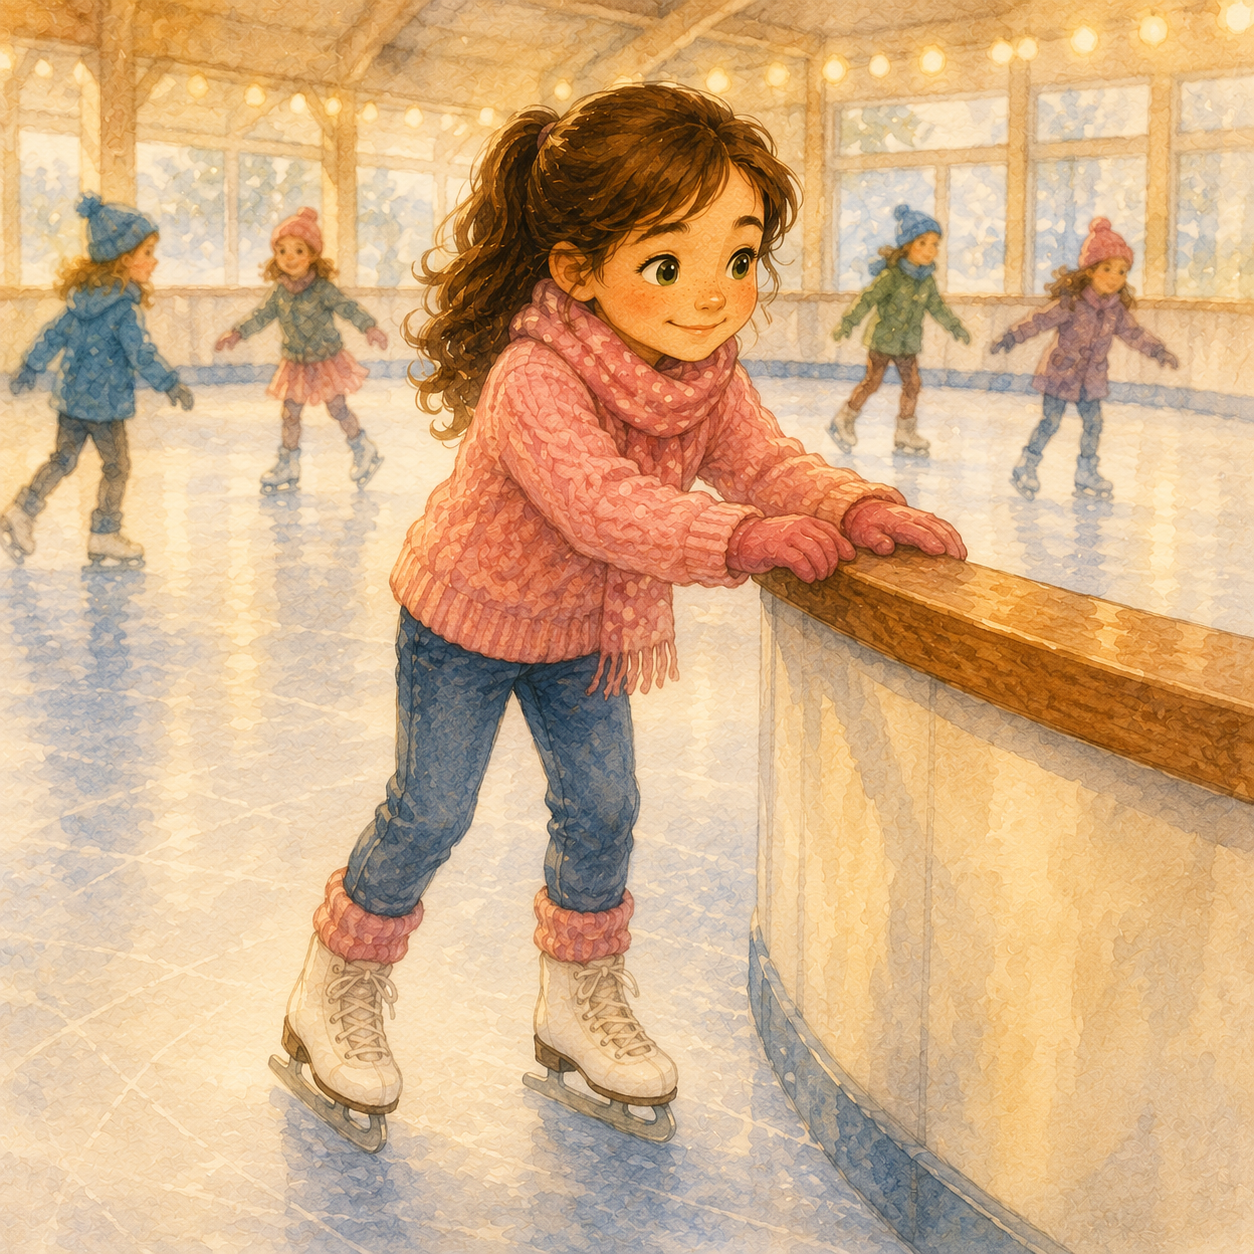
\includegraphics[width=7cm]{img/patinoire.png}
\end{wrapfigure}

Ma grande sœur Émilie fait du patin à glace depuis deux ans. Elle glisse
comme une championne. Un samedi, elle me propose de venir avec elle. «
Tu vas adorer », dit-elle. J'ai un peu peur, mais je dis oui.

Devant la patinoire, il y a une longue file. Quand c'est notre tour, on
me prête une paire de patins. Ils sont blancs, avec de longs lacets.
Émilie serre bien mes lacets. Mes pieds se sentent durs et serrés.

Je marche sur les patins. C'est difficile ! On dirait que je vais tomber
à chaque pas. J'arrive enfin devant la glace. Elle brille comme un
miroir.

Je pose un pied sur la glace. Puis l'autre. Je tiens fort la barrière.
La glace est dure et froide. Je glisse un peu et j'ai très peur.

Émilie, elle, glisse sans effort. Elle tourne, elle recule, elle lève
même une jambe ! Je la regarde, émerveillée. Je voudrais faire pareil.

Émilie revient près de moi. Elle me prend les mains. « Plie un peu les
genoux », dit-elle. J'essaie. Je glisse tout doucement. Je fais quelques
pas. Et puis\ldots{} patatras ! Je tombe sur les fesses. Je ris très
fort. Ce n'est pas grave.

Je me relève toute seule. J'essaie encore. Cette fois, je glisse plus
loin. Petit à petit, je commence à aimer ça.

À la fin de l'heure, je ne veux plus partir. Sur le chemin du retour, je
n'arrête pas d'en parler. Émilie sourit. « Tu sais, dit-elle, il y a un
grand spectacle sur glace cet hiver. Tu pourrais y danser, toi aussi. »

Un spectacle sur glace\ldots{} Et si c'était mon nouveau rêve ?

\begin{center}\rule{0.5\linewidth}{0.5pt}\end{center}

\subsubsection{Questions de
compréhension}\label{questions-de-compruxe9hension-7}

\begin{enumerate}
\def\labelenumi{\arabic{enumi}.}
\tightlist
\item
  Depuis combien de temps Émilie fait-elle du patin ?
\item
  Que ressent Camille la première fois sur la glace ?
\item
  Quel nouveau rêve naît à la fin du chapitre ?
\end{enumerate}

\subsubsection{Mon suivi de lecture}\label{mon-suivi-de-lecture-7}

\begin{center}
\begin{tabularx}{\textwidth}{|X|X|}
\hline
\textbf{Date} & \textbf{Temps} \\
\hline
& \\
\hline
& \\
\hline
& \\
\hline
\end{tabularx}
\end{center}

}% <<FIT END 8>>
\newpage

\sectiondivider{3}{Niveau 2}

\subsubsection{Un peu plus riche}\label{un-peu-plus-riche}

Les chapitres de cette section font environ \textbf{360 mots}. Les
phrases sont un peu plus longues. On y rencontre du \textbf{présent}, de
\textbf{l'imparfait} et du \textbf{passé composé}. Le vocabulaire
devient plus varié.

L'histoire, elle aussi, devient plus riche : la forêt, une grande
frayeur, et un nouveau rêve qui prend forme.

\subsubsection{Combien de temps pour lire un chapitre
?}\label{combien-de-temps-pour-lire-un-chapitre-2}

{\def\LTcaptype{none} % do not increment counter
\begin{longtable}[]{@{}lll@{}}
\toprule\noalign{}
Niveau de référence & Vitesse & Temps pour \textasciitilde360 mots \\
\midrule\noalign{}
\endhead
\bottomrule\noalign{}
\endlastfoot
Fin de CP & 50 mots/min & \textasciitilde7 min 10 s \\
Fin de CE1 & 90 mots/min & \textbf{\textasciitilde{} 4 min} \\
Fin de CE2 & 110 mots/min & \textasciitilde3 min 15 s \\
\end{longtable}
}

\newpage
% <<FIT 9>>
{\storyfont{10}%

\section{Chapitre 9 --- Les habitants de la
forêt}\label{chapitre-9-les-habitants-de-la-foruxeat}

\begin{wrapfigure}{r}{7cm}
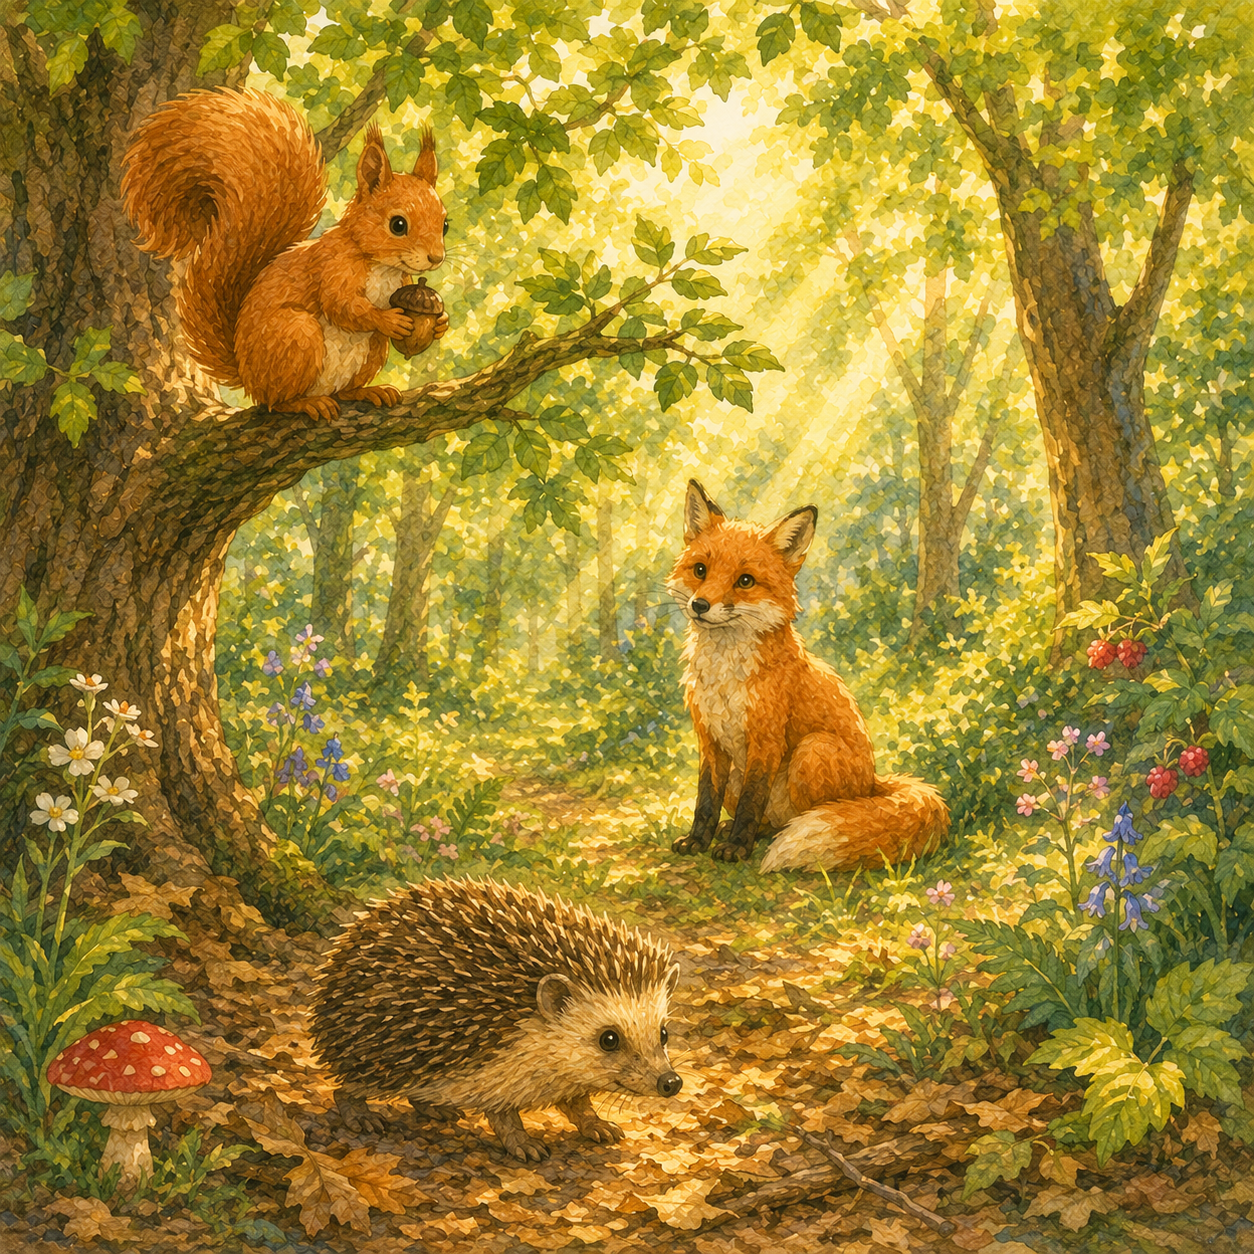
\includegraphics[width=7cm]{img/foret.png}
\end{wrapfigure}

Derrière notre maison, il y a une grande forêt. Un dimanche d'automne,
papa nous y a emmenés en promenade. Mango courait partout, le nez au
sol. Suzanne était venue avec nous, et nous voulions observer les
animaux.

« Pour les voir, a dit papa, il faut être très silencieux. » Alors nous
avons marché sans faire de bruit.

Soudain, Lina a montré quelque chose du doigt. Une petite boule de
piquants, au pied d'un arbre. C'était un hérisson ! Quand Mango s'est
approché, le hérisson s'est mis en boule. Comme cela, personne ne peut
le manger. Papa nous a expliqué qu'il dort le jour et qu'il cherche à
manger la nuit. Il aime les vers de terre, les escargots et les
insectes. En hiver, il dort pendant plusieurs mois : c'est
l'hibernation.

Un peu plus loin, j'ai levé les yeux. Un écureuil roux sautait de
branche en branche. Sa longue queue touffue l'aidait à garder
l'équilibre. Il tenait une noisette dans ses pattes. « En automne, a
chuchoté Suzanne, l'écureuil fait des réserves. » C'est vrai : il cache
des graines un peu partout. Mais il oublie souvent ses cachettes ! Et
ces graines oubliées deviennent parfois de nouveaux arbres.

Enfin, tout au loin, nous avons vu une ombre rousse filer entre les
arbres. « Un renard ! » a murmuré papa. Le renard ressemble un peu à un
petit chien. Il a un beau pelage roux et une queue épaisse. Il chasse
surtout le soir et la nuit. Il vit dans un trou qu'on appelle un
terrier. C'est là qu'il élève ses petits, les renardeaux.

Mango voulait courir derrière le renard. Heureusement, papa le tenait
bien par sa laisse.

Sur le chemin du retour, j'étais très contente. En une seule promenade,
nous avions vu trois animaux de la forêt ! La prochaine fois, je promets
d'ouvrir encore plus grand les yeux et les oreilles.

\begin{center}\rule{0.5\linewidth}{0.5pt}\end{center}

\subsubsection{Questions de
compréhension}\label{questions-de-compruxe9hension-8}

\begin{enumerate}
\def\labelenumi{\arabic{enumi}.}
\tightlist
\item
  Que fait le hérisson quand Mango s'approche ?
\item
  Comment l'écureuil aide-t-il, sans le savoir, à faire pousser de
  nouveaux arbres ?
\item
  Où vit le renard, et comment s'appelle son abri ?
\end{enumerate}

\subsubsection{Mon suivi de lecture}\label{mon-suivi-de-lecture-8}

\begin{center}
\begin{tabularx}{\textwidth}{|X|X|}
\hline
\textbf{Date} & \textbf{Temps} \\
\hline
& \\
\hline
& \\
\hline
& \\
\hline
\end{tabularx}
\end{center}

}% <<FIT END 9>>
\newpage
% <<FIT 10>>
{\storyfont{10}%

\section{Chapitre 10 --- Mango se perd}\label{chapitre-10-mango-se-perd}

\begin{wrapfigure}{r}{7cm}
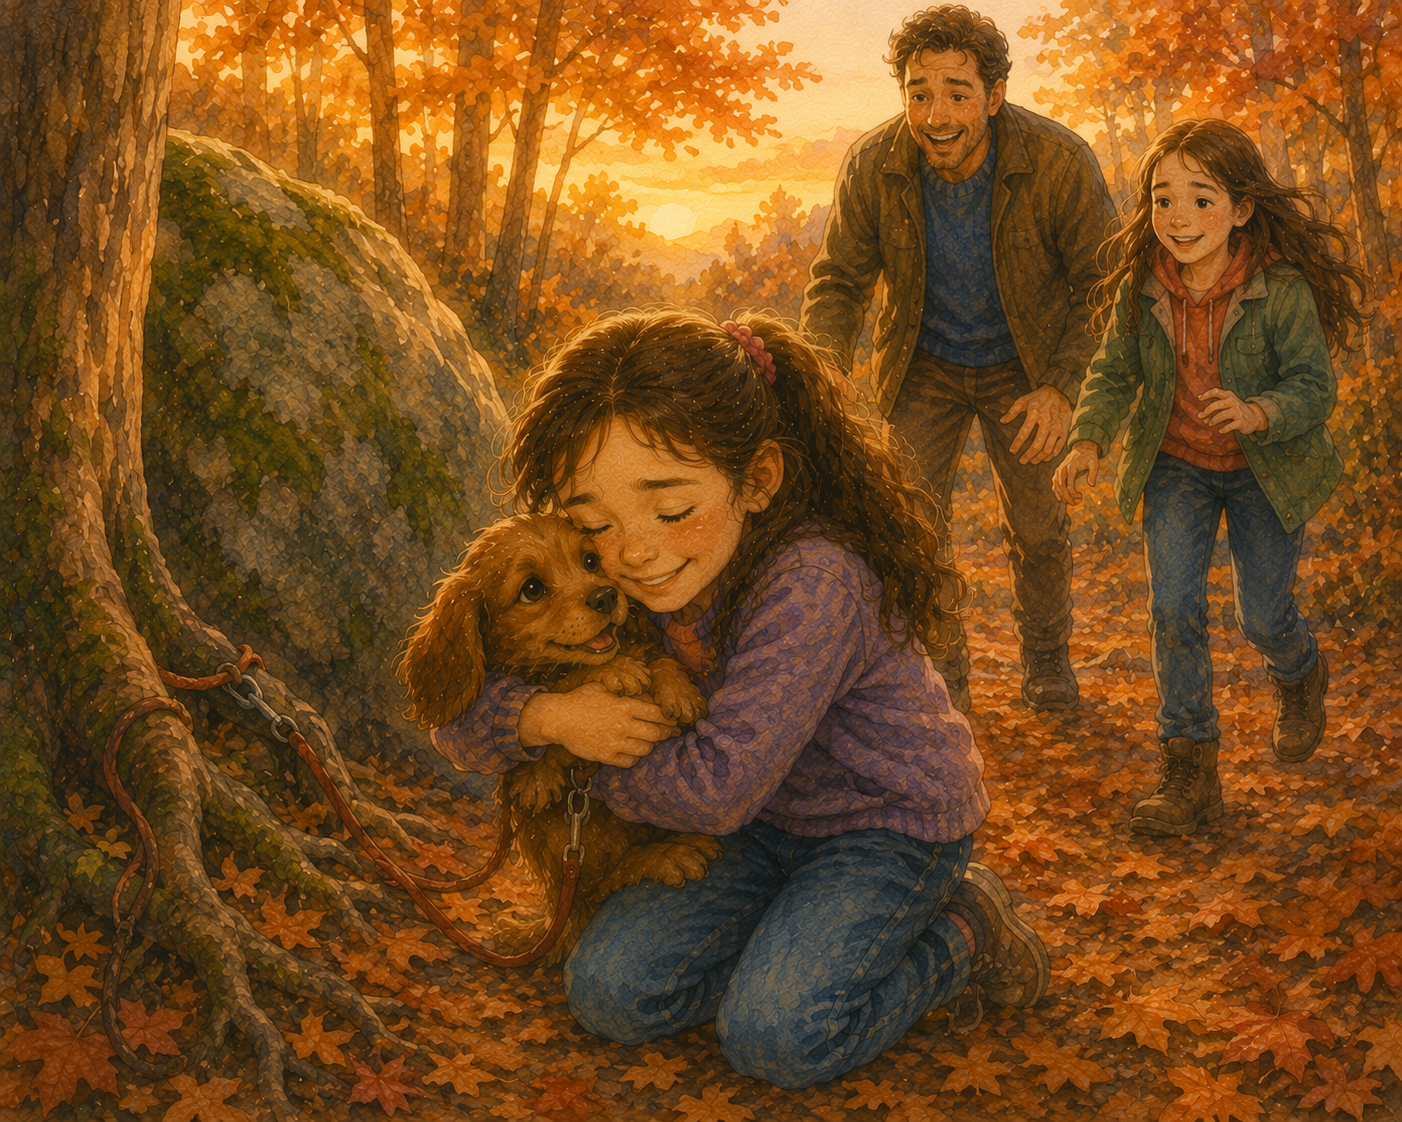
\includegraphics[width=7cm]{img/ch10_perdu.png}
\end{wrapfigure}

Le mercredi suivant, nous sommes retournés dans la forêt. Suzanne était
là, et Mango aussi. Cette fois, papa a laissé Mango courir sans sa
laisse. « Il est sage, maintenant », a-t-il dit.

Au début, tout allait bien. Mango restait près de nous. Il sentait les
feuilles et remuait la queue. Mais soudain, un écureuil a traversé le
chemin. Mango est parti comme une flèche ! Il a couru derrière
l'écureuil, entre les arbres.

« Mango ! Reviens ! » ai-je crié. Mais Mango ne m'écoutait plus. En
quelques secondes, il a disparu.

Nous avons cherché partout. Papa appelait. Suzanne sifflait. Lina
pleurait un peu. Moi, j'avais le cœur serré. La forêt était grande, et
le soir commençait à tomber. Et si Mango ne retrouvait pas son chemin ?
Et s'il avait peur, tout seul dans le noir ?

Nous avons marché longtemps. J'appelais Mango d'une voix tremblante.
Mais rien. Juste le bruit du vent dans les feuilles.

Tout à coup, Suzanne s'est arrêtée. « Écoutez ! » Au loin, on entendait
un petit aboiement. Nous avons couru vers le bruit. Et là, près d'un
grand rocher, nous avons trouvé Mango. Il était coincé : sa laisse
s'était accrochée à une racine. Il tirait, mais il ne pouvait plus
avancer.

Quand Mango m'a vue, il a remué la queue très fort. Il a poussé des
petits cris de joie. Doucement, papa a libéré sa laisse. J'ai pris Mango
dans mes bras. Il tremblait un peu, mais il allait bien. Je l'ai serré
très fort.

« Tu m'as fait tellement peur », lui ai-je murmuré.

Sur le chemin du retour, Mango est resté tout près de moi. Je crois
qu'il avait compris la leçon. Et moi aussi : dans la forêt, on garde
toujours son chien près de soi.

Ce soir-là, Mango s'est endormi contre mon lit. Et pour la première
fois, papa l'a laissé dormir dans ma chambre.

\begin{center}\rule{0.5\linewidth}{0.5pt}\end{center}

\subsubsection{Questions de
compréhension}\label{questions-de-compruxe9hension-9}

\begin{enumerate}
\def\labelenumi{\arabic{enumi}.}
\tightlist
\item
  Pourquoi Mango part-il soudain en courant ?
\item
  Comment la famille finit-elle par retrouver Mango ?
\item
  Quelle leçon Camille a-t-elle apprise ce jour-là ?
\end{enumerate}

\subsubsection{Mon suivi de lecture}\label{mon-suivi-de-lecture-9}

\begin{center}
\begin{tabularx}{\textwidth}{|X|X|}
\hline
\textbf{Date} & \textbf{Temps} \\
\hline
& \\
\hline
& \\
\hline
& \\
\hline
\end{tabularx}
\end{center}

}% <<FIT END 10>>
\newpage
% <<FIT 11>>
{\storyfont{11}%

\section{Chapitre 11 --- Camille
s'entraîne}\label{chapitre-11-camille-sentrauxeene}

\begin{wrapfigure}{r}{7cm}
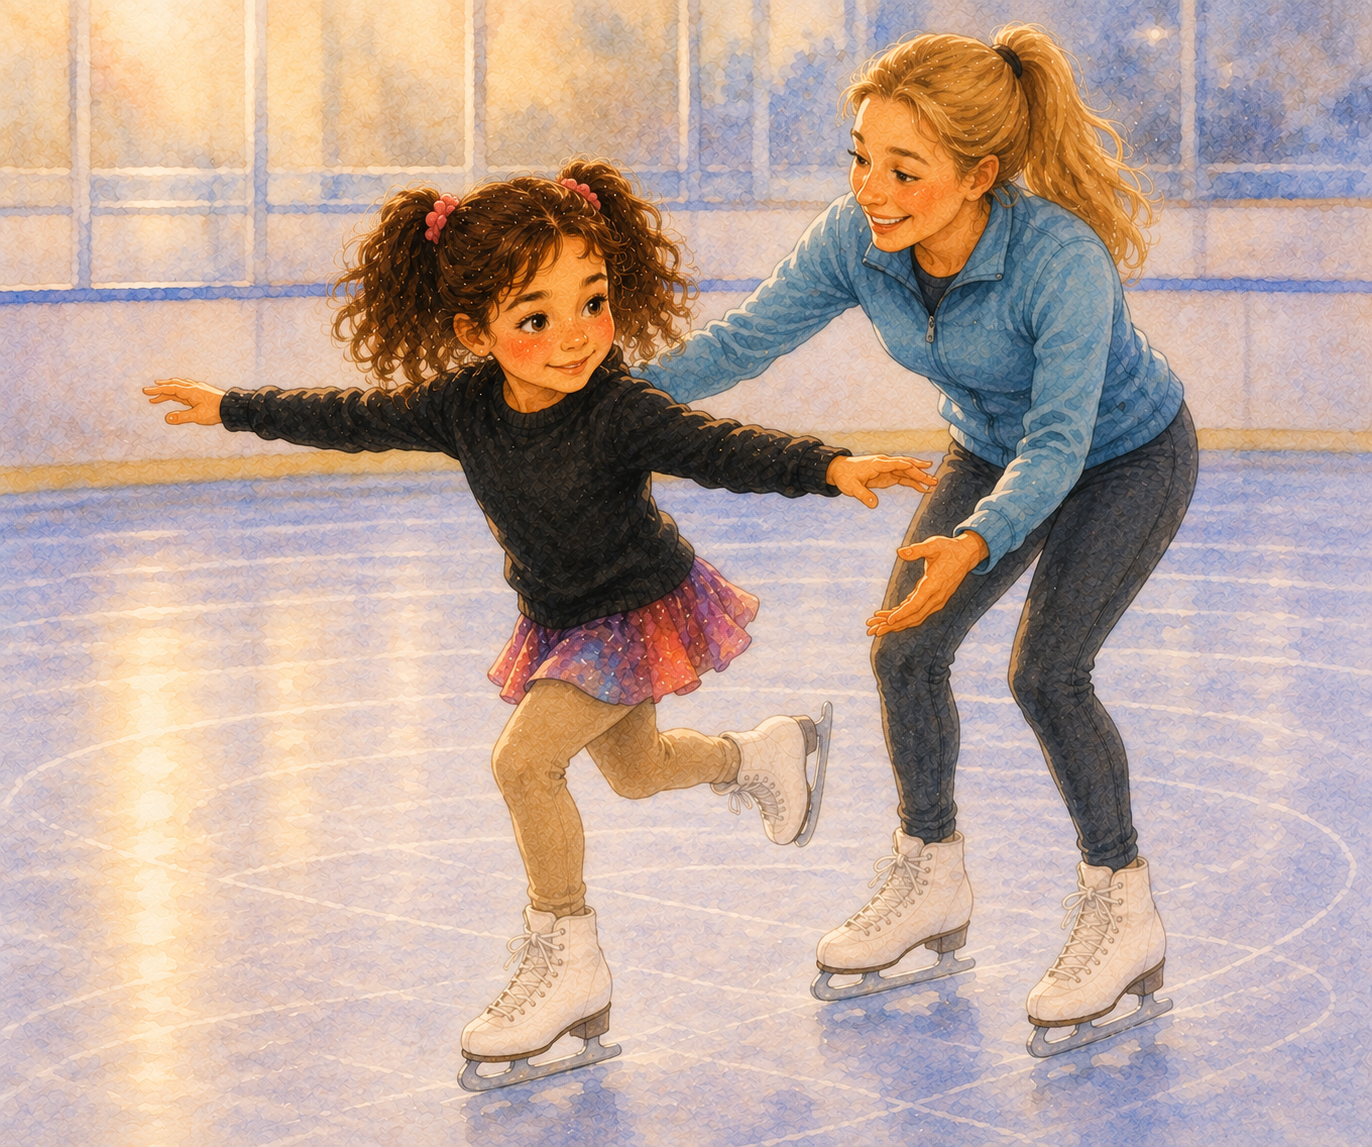
\includegraphics[width=7cm]{img/ch11_entrainement.png}
\end{wrapfigure}

Depuis ma première fois sur la glace, je n'avais plus qu'une idée en
tête : danser au grand spectacle d'hiver. Émilie m'avait dit que c'était
possible. Alors j'ai demandé à maman de m'inscrire à des cours de
patinage.

Mon professeur s'appelle Loïcia. Elle est patiente et très gentille. Au
premier cours, j'avais encore peur de tomber. Loïcia m'a pris la main. «
Sur la glace, a-t-elle dit, on tombe tous. Ce qui compte, c'est de se
relever. »

Chaque samedi, je vais à la patinoire. Au début, c'était difficile. Je
tombais souvent. Mes jambes tremblaient. Mais petit à petit, j'ai
progressé. Maintenant, je sais glisser sur un pied. Je sais tourner. Je
sais même reculer un peu.

À la maison aussi, je m'entraîne. Dans le jardin, je fais semblant de
patiner sur l'herbe. Émilie me montre les bons gestes : le dos droit,
les genoux pliés, les bras ouverts. Mango, lui, court autour de moi en
aboyant. Il croit que c'est un jeu !

Certains jours, j'ai envie d'abandonner. Un samedi, je suis tombée très
fort. J'avais mal et j'avais un peu honte. Je ne voulais plus y
retourner. Mais le soir, Émilie est venue dans ma chambre. « Quand j'ai
commencé, m'a-t-elle dit, je tombais encore plus que toi. Ne lâche pas.
» Ses mots m'ont redonné du courage.

Les semaines ont passé. Les feuilles sont tombées. Le froid est arrivé.
Et moi, je patinais de mieux en mieux.

Un jour, Loïcia m'a appelée après le cours. « Camille, j'ai une question
pour toi. Veux-tu danser au spectacle d'hiver ? » Mon cœur a fait un
bond. « Oh oui ! » ai-je répondu.

À partir de ce jour, j'ai travaillé encore plus fort. Je préparais mon
numéro. Loïcia choisissait une jolie musique. Le grand jour approchait.
J'étais à la fois très heureuse et un peu effrayée.

\begin{center}\rule{0.5\linewidth}{0.5pt}\end{center}

\subsubsection{Questions de
compréhension}\label{questions-de-compruxe9hension-10}

\begin{enumerate}
\def\labelenumi{\arabic{enumi}.}
\tightlist
\item
  Comment s'appelle le professeur de patinage de Camille ?
\item
  Que fait Camille pour s'entraîner à la maison ?
\item
  Qui lui redonne du courage après une grosse chute ?
\end{enumerate}

\subsubsection{Mon suivi de lecture}\label{mon-suivi-de-lecture-10}

\begin{center}
\begin{tabularx}{\textwidth}{|X|X|}
\hline
\textbf{Date} & \textbf{Temps} \\
\hline
& \\
\hline
& \\
\hline
& \\
\hline
\end{tabularx}
\end{center}

}% <<FIT END 11>>
\newpage
% <<FIT 12>>
{\storyfont{10}%

\section{Chapitre 12 --- Médor, le chien
héros}\label{chapitre-12-muxe9dor-le-chien-huxe9ros}

\begin{wrapfigure}{r}{7cm}
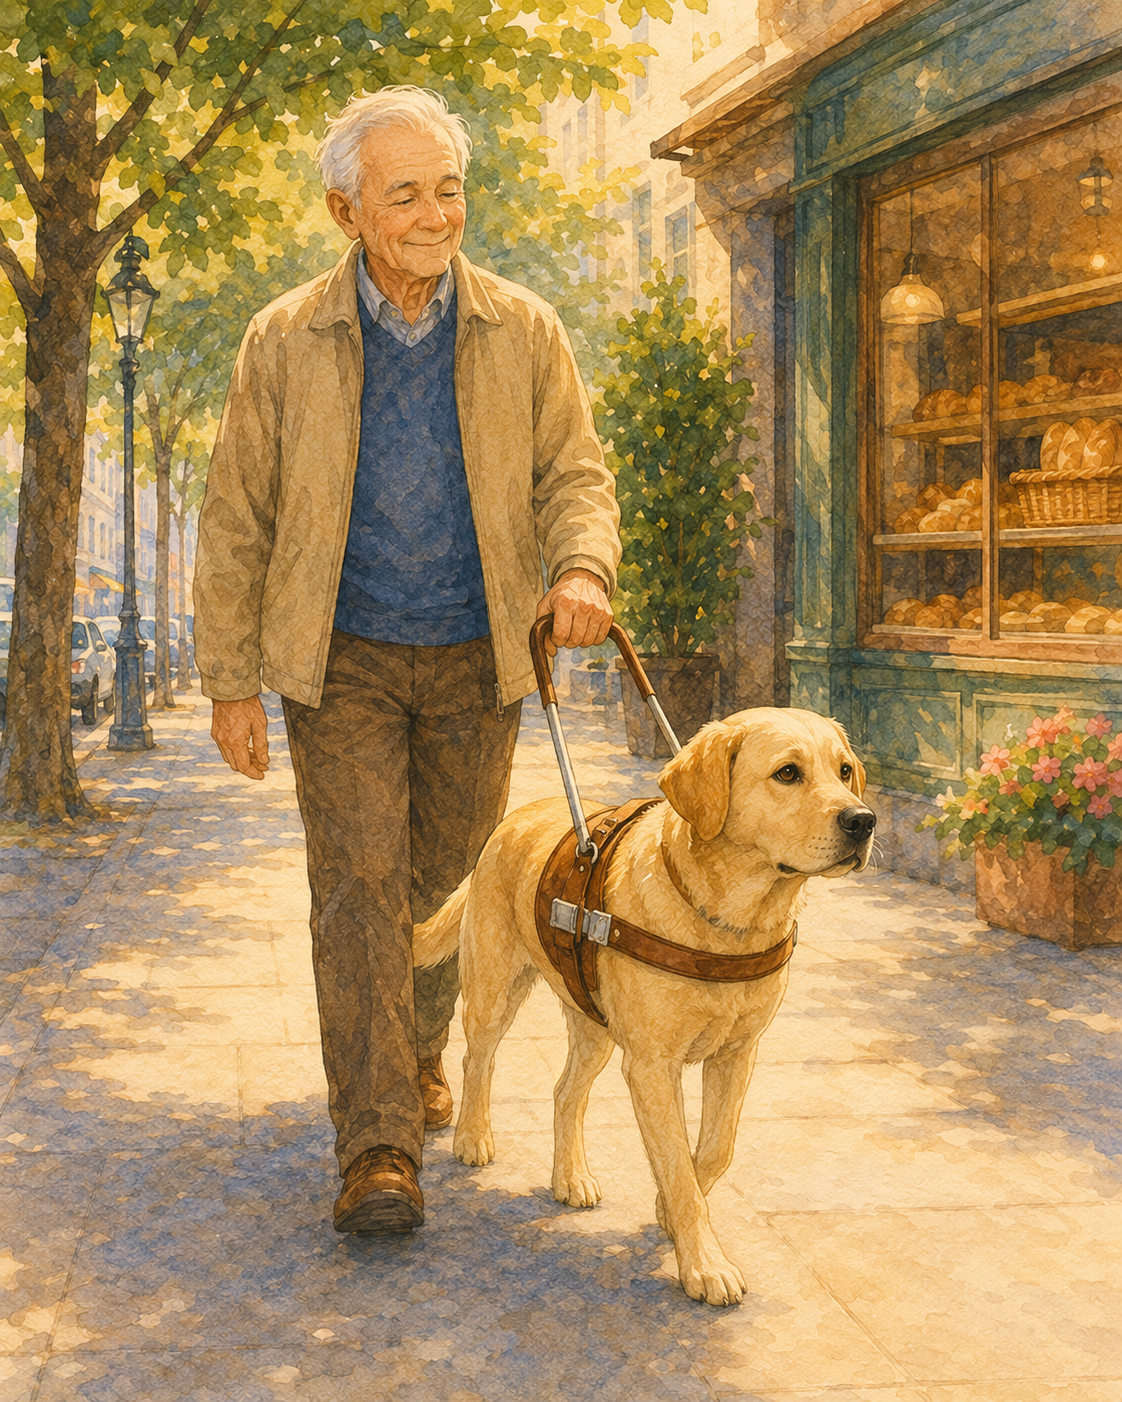
\includegraphics[width=7cm]{img/medor.png}
\end{wrapfigure}

Un dimanche, au parc, nous avons rencontré un monsieur avec un grand
chien. Le monsieur s'appelle Léon. Il a soixante ans. Son chien
s'appelle Médor.

Tout de suite, Mango a voulu jouer avec Médor. Mais Léon a dit : «
Attends un peu. Médor travaille, en ce moment. » J'étais étonnée. Un
chien qui travaille ?

Léon nous a expliqué. Il est aveugle : il ne voit rien, ni la lumière,
ni les couleurs. Médor est un chien guide. Son travail, c'est d'aider
Léon à se déplacer partout : dans la rue, dans les magasins, dans le
bus.

Médor portait une sorte de petite ceinture spéciale : le harnais. «
Quand Médor porte son harnais, a dit Léon, il sait qu'il est au travail.
Il devient très sérieux. »

Médor sait faire des choses extraordinaires. Quand il y a une marche, il
s'arrête. Quand quelqu'un arrive en face, il se déplace sur le côté.
Quand une voiture approche, il s'arrête et refuse d'avancer, même si
Léon le lui demande. Comme cela, Léon ne risque rien.

« Comment Médor a-t-il appris tout ça ? » a demandé Lina. Léon a souri.
« Dans une école spéciale, pendant deux ans. Il a travaillé très dur. »

Deux ans d'efforts ! J'ai pensé à mon patinage. Moi aussi, je
travaillais dur pour y arriver. Si Médor avait réussi, alors je pouvais
réussir, moi aussi.

Ensuite, Léon a enlevé le harnais. « Maintenant, Médor n'est plus au
travail. » D'un coup, Médor est devenu un chien comme les autres. Il a
couru, il a joué avec Mango, il a fait la fête à tout le monde.

Avant de partir, Léon m'a dit une chose que je n'oublierai jamais : «
Avec de la patience et du travail, on peut apprendre presque tout. »

Cette nuit-là, j'ai rêvé de la glace. Le spectacle approchait. Et grâce
à Médor, je me sentais plus forte.

\begin{center}\rule{0.5\linewidth}{0.5pt}\end{center}

\subsubsection{Questions de
compréhension}\label{questions-de-compruxe9hension-11}

\begin{enumerate}
\def\labelenumi{\arabic{enumi}.}
\tightlist
\item
  Quel est le travail de Médor ?
\item
  Combien de temps a duré l'apprentissage de Médor ?
\item
  Quelle phrase de Léon donne du courage à Camille ?
\end{enumerate}

\subsubsection{Mon suivi de lecture}\label{mon-suivi-de-lecture-11}

\begin{center}
\begin{tabularx}{\textwidth}{|X|X|}
\hline
\textbf{Date} & \textbf{Temps} \\
\hline
& \\
\hline
& \\
\hline
& \\
\hline
& \\
\hline
& \\
\hline
\end{tabularx}
\end{center}

}% <<FIT END 12>>
\newpage

\sectiondivider{4}{Niveau 3}

\subsubsection{Niveau CE1 complet}\label{niveau-ce1-complet}

Les chapitres de cette section font environ \textbf{450 mots}. C'est le
niveau attendu en fin de CE1. Le vocabulaire est plus riche, les phrases
peuvent aller jusqu'à 18 mots, et tu rencontreras toutes les
conjugaisons courantes (présent, imparfait, passé composé, futur).

C'est aussi la fin de l'histoire : un grand voyage, le retour des
saisons, et le moment que Camille attend depuis si longtemps.

\subsubsection{Combien de temps pour lire un chapitre
?}\label{combien-de-temps-pour-lire-un-chapitre-3}

{\def\LTcaptype{none} % do not increment counter
\begin{longtable}[]{@{}lll@{}}
\toprule\noalign{}
Niveau de référence & Vitesse & Temps pour \textasciitilde450 mots \\
\midrule\noalign{}
\endhead
\bottomrule\noalign{}
\endlastfoot
Fin de CP & 50 mots/min & \textasciitilde9 min \\
Fin de CE1 & 90 mots/min & \textbf{\textasciitilde{} 5 min} \\
Fin de CE2 & 110 mots/min & \textasciitilde4 min 05 s \\
\end{longtable}
}

\newpage
% <<FIT 13>>
{\storyfont{11}%

\section{Chapitre 13 --- Le voyage en
Écosse}\label{chapitre-13-le-voyage-en-uxe9cosse}

\begin{wrapfigure}{r}{7cm}
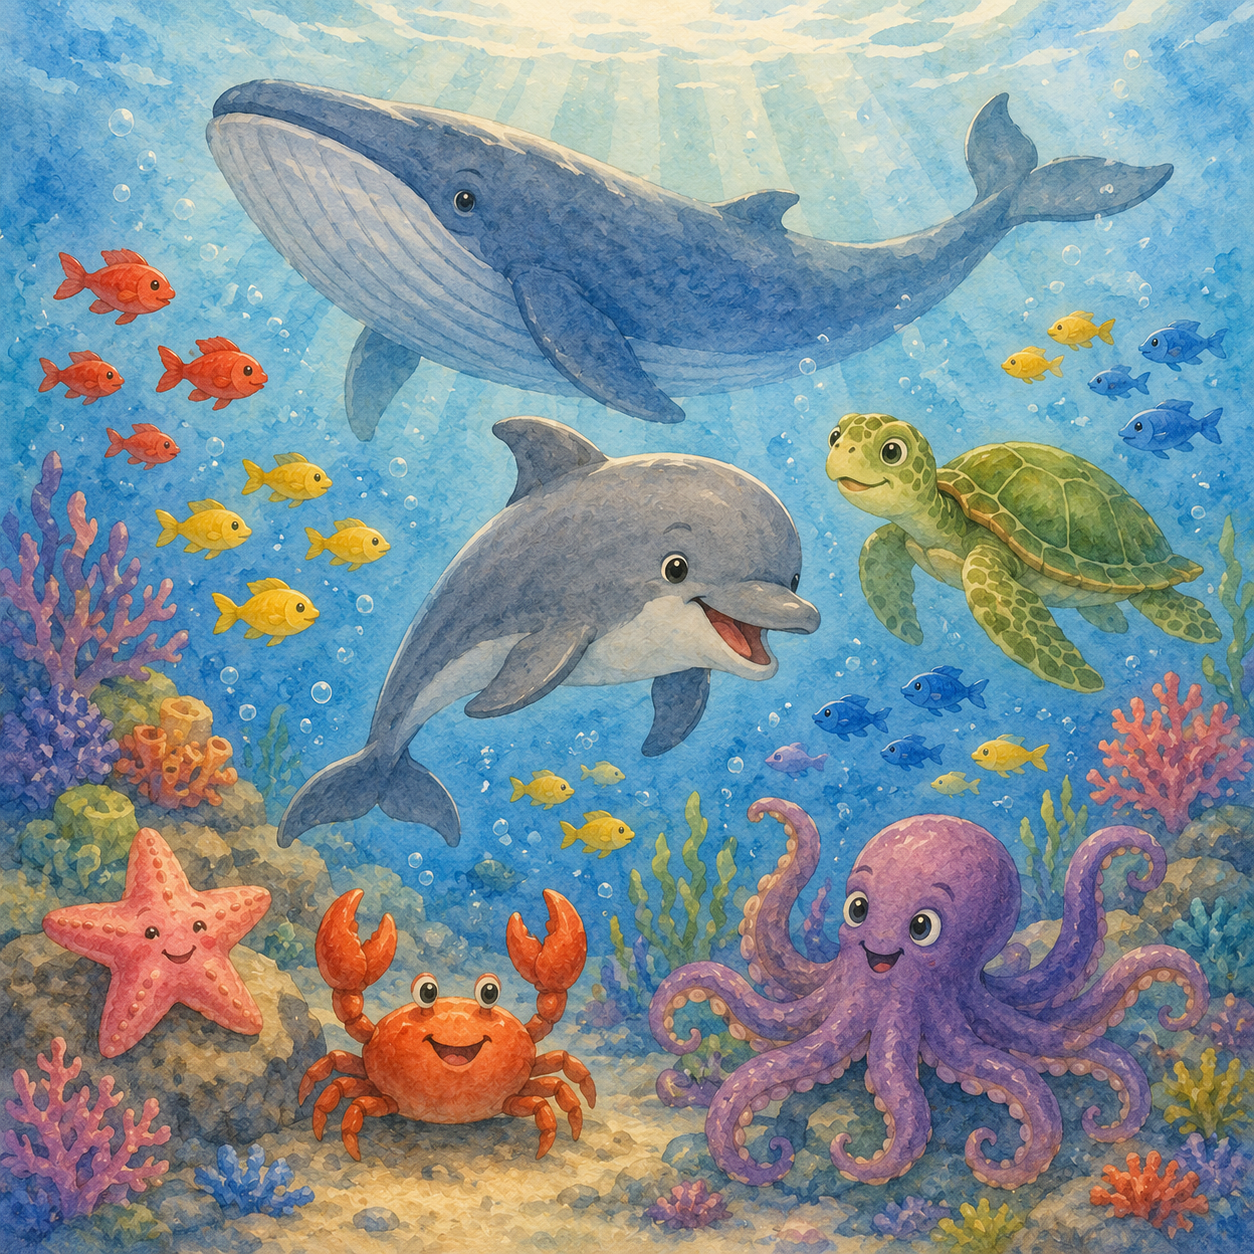
\includegraphics[width=7cm]{img/mer.png}
\end{wrapfigure}

Pendant les vacances, nous sommes partis en voyage, tous les cinq. Notre
destination : l'Écosse, un pays tout au nord, à côté de l'Angleterre.
Mango, lui, est resté chez Suzanne. J'étais un peu triste de le laisser,
mais Suzanne m'a promis de bien s'en occuper.

L'Écosse est un pays magnifique et un peu mystérieux. Il y pleut
souvent, alors tout est très vert. On appelle les grandes collines
vertes les Highlands. Là-bas, le vent souffle fort et les nuages courent
dans le ciel.

Le premier jour, nous avons visité un vieux château en pierre, posé en
haut d'une colline. À l'intérieur, il faisait froid et sombre. Papa nous
a raconté des histoires de fantômes. Lina avait un peu peur, mais moi,
j'adorais ça.

Le lendemain, nous avons longé un grand lac, très long et très profond.
En Écosse, on dit un « loch ». Maman nous a raconté la légende : on dit
qu'un monstre vivrait au fond de ce lac ! Émilie et moi, nous avons
scruté l'eau pendant longtemps. Mais nous n'avons rien vu\ldots{} sauf
des canards.

Sur la route, nous avons croisé des moutons partout. Nous avons aussi vu
de drôles de vaches rousses, avec de longs poils et de grandes cornes :
les vaches des Highlands. Une fois, au bord d'un bois, un grand cerf
nous a regardés passer. Il portait des bois magnifiques sur la tête.

Mais le plus beau, c'était la promenade en bateau. Nous sommes montés
sur un petit bateau pour aller voir les animaux de la mer. D'abord, des
dauphins ont nagé tout près de nous. Ils sautaient hors de l'eau, comme
pour jouer ! Ensuite, nous avons vu des phoques couchés sur les rochers.
Ils étaient gros et paresseux, au soleil.

Tout à coup, le guide a crié : « Une baleine ! » Au loin, un grand dos
gris est sorti de l'eau. C'était bien une baleine ! Le guide nous a
expliqué qu'elle mange du krill : de minuscules crevettes des mers
froides. Je n'oublierai jamais ce moment.

Le soir, à l'hôtel, j'ai écrit une carte à Suzanne. « Tu ne devineras
jamais tout ce que j'ai vu ! »

Demain, nous rentrerons à la maison. Je serai très contente de retrouver
Mango. Mais ce voyage en Écosse, je m'en souviendrai toute ma vie.

\begin{center}\rule{0.5\linewidth}{0.5pt}\end{center}

\subsubsection{Questions de
compréhension}\label{questions-de-compruxe9hension-12}

\begin{enumerate}
\def\labelenumi{\arabic{enumi}.}
\tightlist
\item
  Pourquoi Mango ne part-il pas en voyage avec la famille ?
\item
  Quelle légende raconte-t-on à propos du loch ?
\item
  Quels animaux la famille voit-elle pendant la promenade en bateau ?
\end{enumerate}

\begin{center}\rule{0.5\linewidth}{0.5pt}\end{center}

}% <<FIT END 13>>
\newpage
% <<FIT 14>>
{\storyfont{11}%

\section{Chapitre 14 --- Les quatre saisons de la
forêt}\label{chapitre-14-les-quatre-saisons-de-la-foruxeat}

\begin{wrapfigure}{r}{7cm}
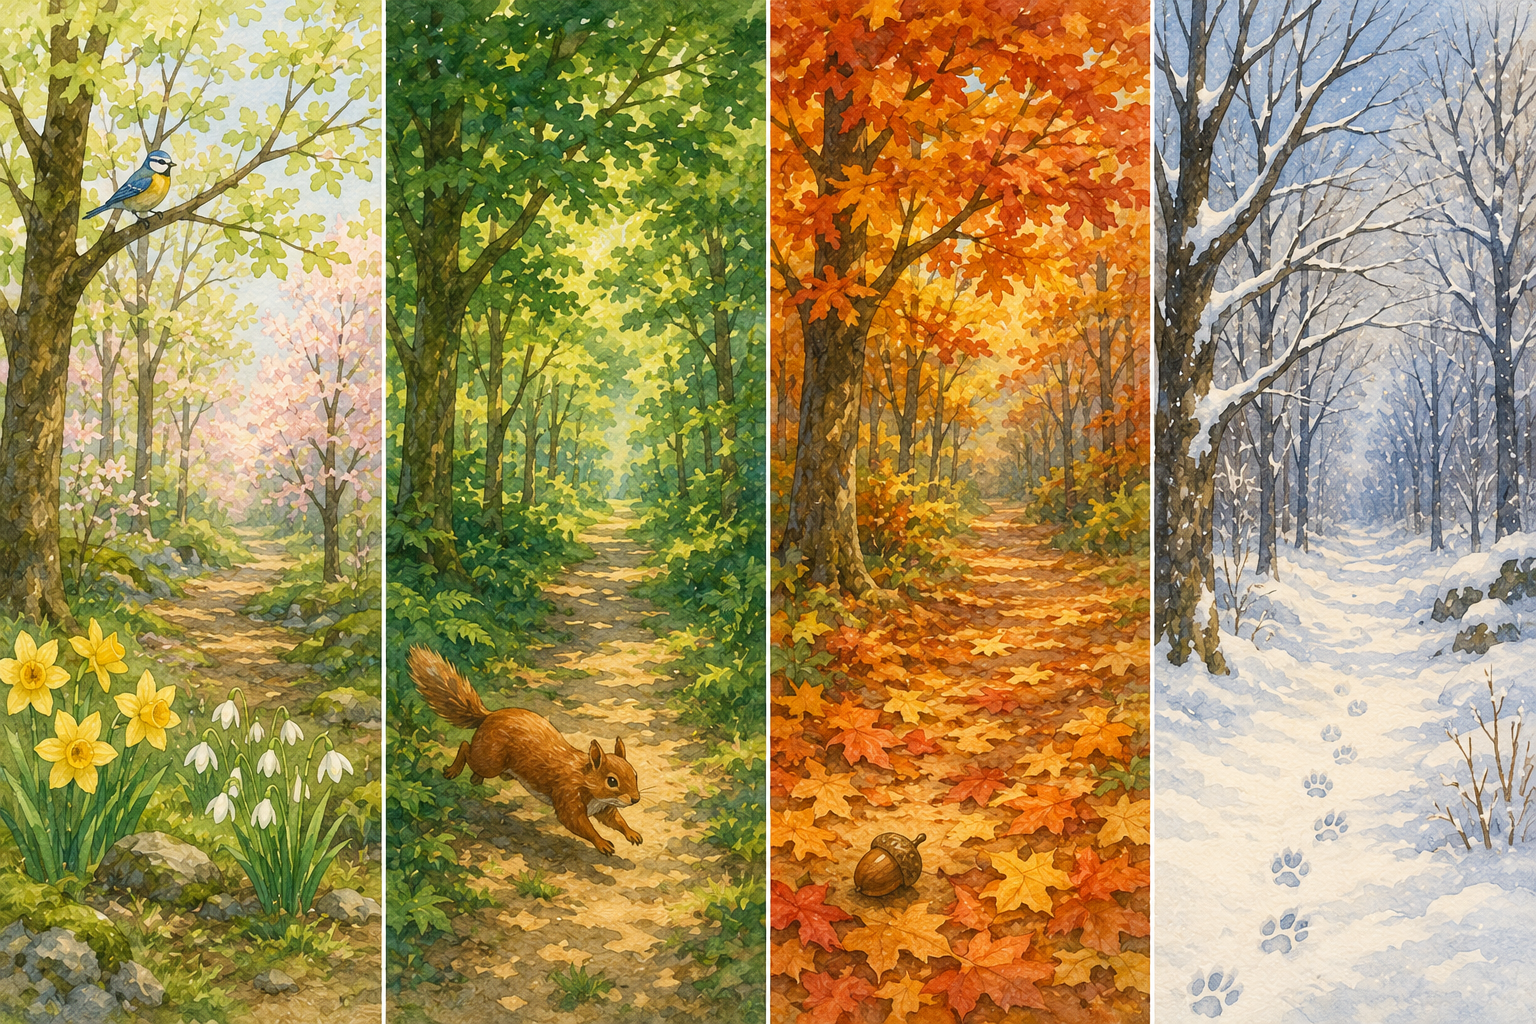
\includegraphics[width=7cm]{img/saisons.png}
\end{wrapfigure}

De retour à la maison, j'ai retrouvé Mango. Quelle joie ! Il a sauté
partout et m'a léché tout le visage. L'hiver approchait, et avec lui, le
grand spectacle. En attendant, j'aimais me promener dans la forêt et
regarder comme elle avait changé depuis le printemps.

Car la forêt n'est jamais la même. Elle change tout au long de l'année.
Chaque saison apporte ses couleurs, ses odeurs et ses bruits.

Au printemps, quand Mango est arrivé chez nous, la forêt se réveillait.
Les arbres faisaient de petites feuilles toutes neuves, d'un vert très
clair. Le sol se couvrait de fleurs : des jonquilles jaunes, des
violettes, des perce-neige. Les oiseaux chantaient dès le matin. C'était
la saison des bébés animaux : les renardeaux et les jeunes chevreuils
étaient nés à ce moment-là.

En été, quand nous avons planté les radis, la forêt était toute verte.
Les feuilles étaient grandes et faisaient de l'ombre. Quand il faisait
très chaud dehors, il faisait plus frais sous les arbres. Les animaux se
cachaient le jour et sortaient le soir. Sur les buissons, les mûres et
les framboises commençaient à mûrir.

En automne, quand Mango s'est perdu, la forêt changeait de couleur. Les
feuilles passaient du vert au jaune, puis à l'orange et au rouge. Quand
on marchait dessus, ça faisait « crac crac ». Les écureuils étaient très
occupés : ils faisaient leurs réserves pour l'hiver. Des champignons
poussaient un peu partout. Mais attention : il ne faut jamais ramasser
un champignon tout seul, car certains sont très dangereux.

Et maintenant, c'est l'hiver. La forêt est calme et silencieuse. Les
arbres ont perdu toutes leurs feuilles. Les branches sont nues et
noires. Parfois, la neige les recouvre, et tout devient blanc.

Beaucoup d'animaux dorment pendant l'hiver. Les hérissons hibernent. Ils
ne se réveilleront qu'au printemps. D'autres, comme les renards, restent
éveillés, mais ils ont du mal à trouver à manger.

Hier, dans la neige, j'ai vu des traces de pas. Ces empreintes
racontaient tous les animaux passés par là pendant la nuit. Mango les
sentait avec son nez.

Une année entière s'est écoulée depuis l'arrivée de Mango. Et bientôt,
sur la glace, ce sera mon grand jour.

\begin{center}\rule{0.5\linewidth}{0.5pt}\end{center}

\subsubsection{Questions de
compréhension}\label{questions-de-compruxe9hension-13}

\begin{enumerate}
\def\labelenumi{\arabic{enumi}.}
\tightlist
\item
  Quelle saison est la saison des bébés animaux ?
\item
  Pourquoi ne faut-il jamais ramasser un champignon tout seul ?
\item
  Que racontent les traces de pas dans la neige ?
\end{enumerate}

\begin{center}\rule{0.5\linewidth}{0.5pt}\end{center}

}% <<FIT END 14>>
\newpage
% <<FIT 15>>
{\storyfont{10}%

\section{Chapitre 15 --- Le grand spectacle sur
glace}\label{chapitre-15-le-grand-spectacle-sur-glace}

\begin{wrapfigure}{r}{7cm}
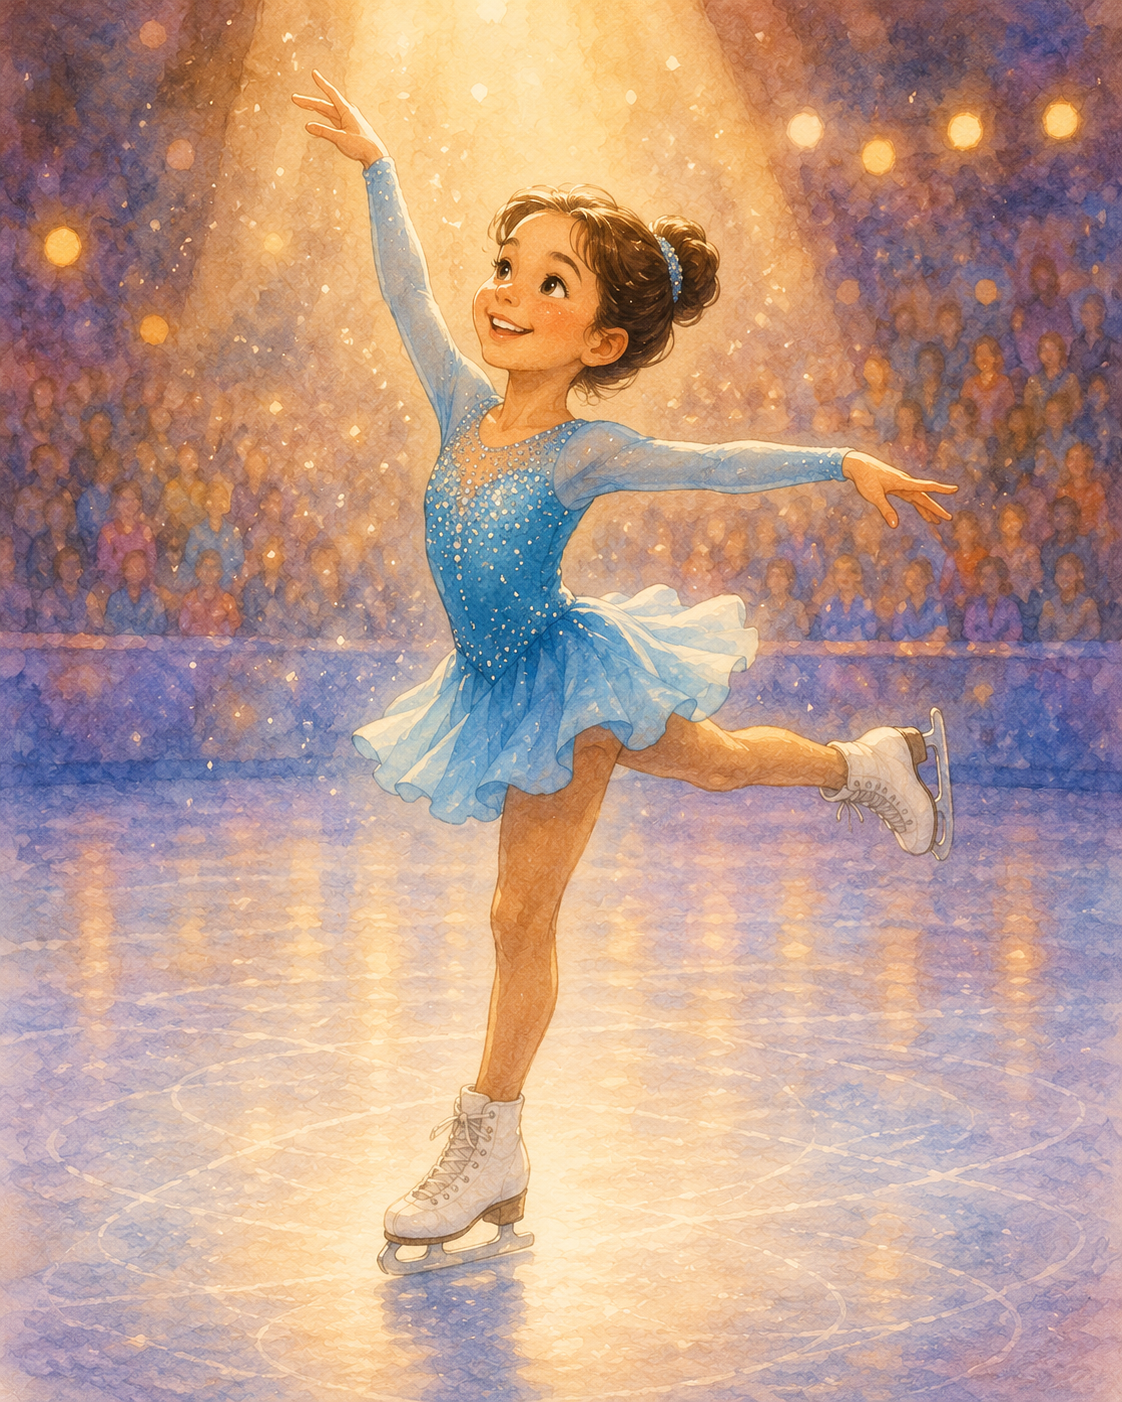
\includegraphics[width=7cm]{img/spectacle.png}
\end{wrapfigure}

Ce soir, c'est le grand jour. Je vais danser sur la glace devant tout le
monde. Depuis des mois, je m'entraîne avec Loïcia. Elle dit que je suis
prête. Mais moi, je ne suis pas si sûre.

Dans les vestiaires, beaucoup d'enfants se préparent. J'ai mis ma jolie
robe bleue. Maman m'a coiffée avec un chignon et m'a mis un peu de
paillettes sur les joues. Je me regarde dans le miroir : on dirait une
vraie patineuse !

Loïcia nous rassemble. « Souriez et amusez-vous, nous dit-elle. C'est
tout ce que je vous demande. » Mais mon ventre fait des nœuds.

La salle est pleine. Quelque part dans le public, il y a toute ma
famille : papa, maman, Lina et Émilie. Suzanne est venue, elle aussi. Et
il y a une belle surprise : Léon est là, avec Médor couché bien sagement
à ses pieds. Ils sont tous venus pour moi.

La musique commence. Mon groupe entre sur la glace. Je suis la
troisième. Quand mon tour arrive, mes jambes tremblent. Je pose un patin
sur la glace, puis l'autre. La lumière est très forte. Tout le monde me
regarde.

Je commence à patiner. Au début, je pense à tout : les genoux pliés, le
dos droit, le sourire. Mais peu à peu, j'oublie le public. Je suis dans
la musique. Mes pieds glissent tout seuls. Je tourne sur moi-même comme
une toupie. Je fais ma figure préférée : un grand cercle, avec un pied
levé en l'air.

À un moment, je glisse un peu trop et je manque de tomber. Mais je me
souviens des mots de Loïcia : « On tombe tous ; ce qui compte, c'est de
tenir bon. » Alors je garde l'équilibre. Je continue à sourire. Le
public ne voit rien.

À la fin de la musique, je m'arrête au milieu de la glace. Je lève les
bras vers le ciel. Tout le monde applaudit très fort. J'entends même
quelqu'un crier « Bravo Camille ! » C'est Lina, c'est sûr.

Quand je sors de la glace, Émilie me serre dans ses bras. « Tu as été
parfaite, comme une grande ! » Maman pleure un peu, mais c'est de joie.
Suzanne saute partout. Et Médor remue la queue, comme s'il avait tout
compris.

Je ne sais pas si je serai une grande patineuse, plus tard. Mais ce
soir, je suis la patineuse la plus heureuse du monde. Et tout ça, grâce
au travail, au courage\ldots{} et à tous ceux que j'aime.

\begin{center}\rule{0.5\linewidth}{0.5pt}\end{center}

\subsubsection{Questions de
compréhension}\label{questions-de-compruxe9hension-14}

\begin{enumerate}
\def\labelenumi{\arabic{enumi}.}
\tightlist
\item
  Qui est venu dans le public pour voir Camille ?
\item
  Que se passe-t-il quand Camille glisse un peu trop pendant son numéro
  ?
\item
  À qui Camille dit-elle merci, à la fin ?
\end{enumerate}

\begin{center}\rule{0.5\linewidth}{0.5pt}\end{center}

}% <<FIT END 15>>
\newpage
% <<FIT 16>>
{\storyfont{10}%

\section{Chapitre 16 --- Lettre à
Mamie}\label{chapitre-16-lettre-uxe0-mamie}

\begin{wrapfigure}{r}{7cm}
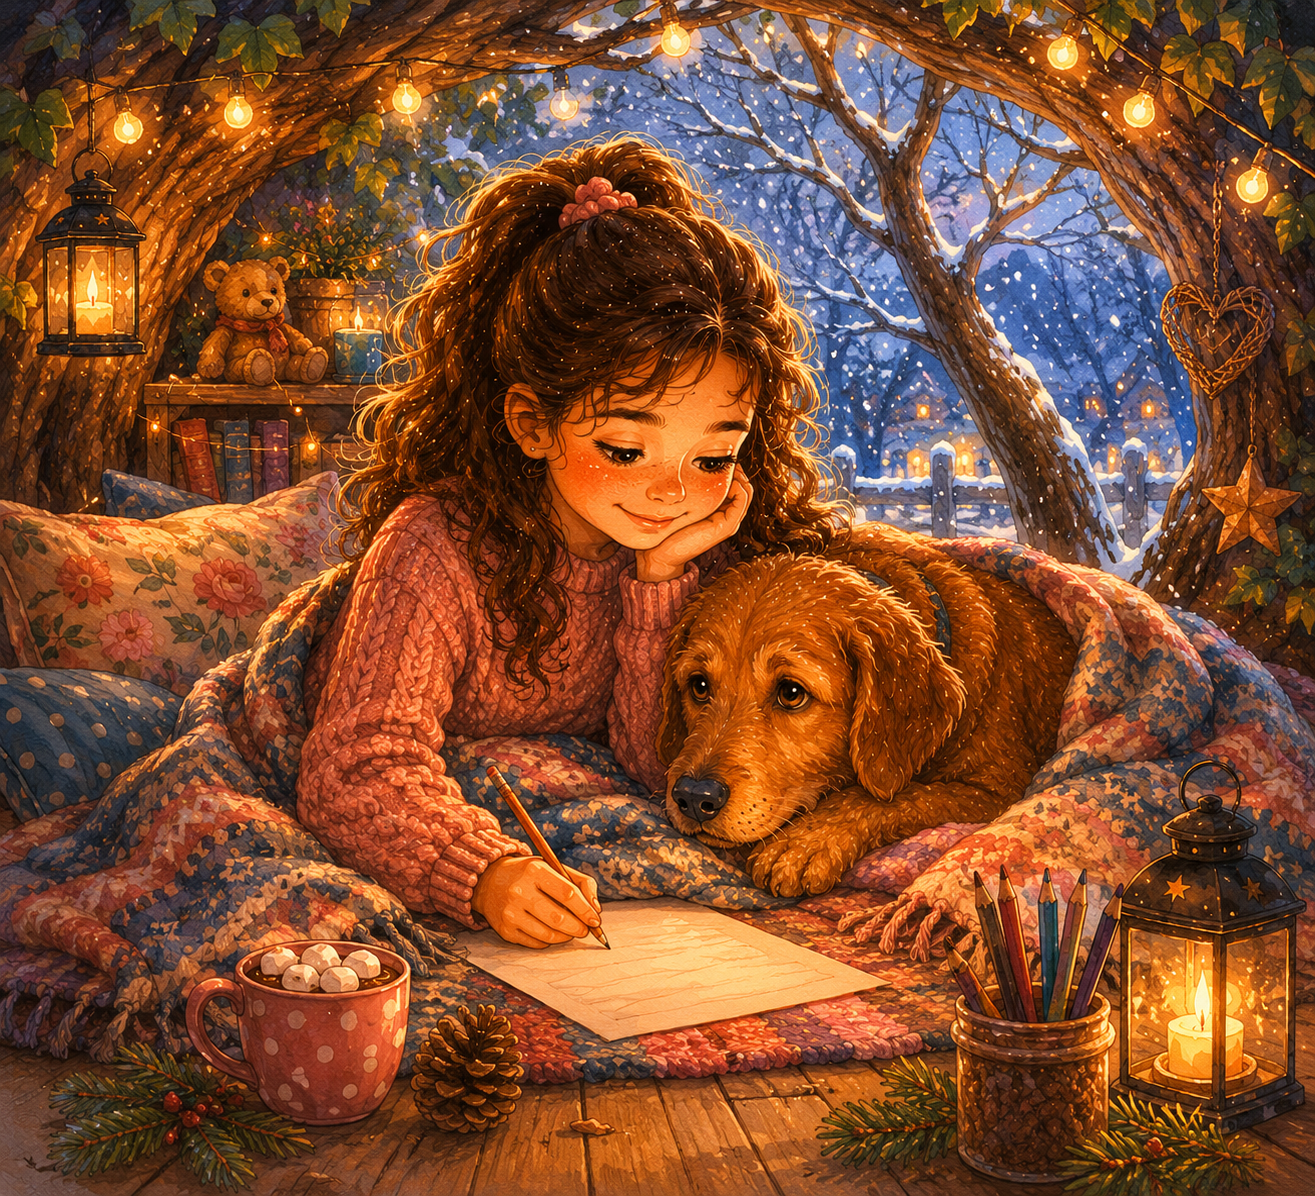
\includegraphics[width=7cm]{img/ch16_lettre.png}
\end{wrapfigure}

Chère Mamie,

Je t'écris de ma cabane secrète, au fond du jardin. Il fait froid, mais
je suis bien au chaud sous une couverture, avec Mango couché contre moi.
J'ai tant de choses à te raconter ! Cette année a été la plus belle de
ma vie.

Tu te souviens, au printemps, je rêvais d'avoir un chien. Eh bien, mon
rêve s'est réalisé ! Mango est arrivé à la maison. C'est un petit chien
tout brun, avec de grandes oreilles. Au début, il était minuscule.
Maintenant, il a bien grandi. Il court partout et il adore le jardin.
C'est mon meilleur ami à quatre pattes.

Avec Mango, on a vécu plein d'aventures. Les jours de pluie, on jouait
aux explorateurs dans ma cabane secrète. On a planté des radis (il les a
tous déterrés, ce coquin !). On a exploré la forêt derrière la maison.
Un jour, Mango s'est perdu et j'ai eu très peur. Heureusement, on l'a
vite retrouvé. Depuis, il dort dans ma chambre.

Cet été, nous sommes aussi partis en Écosse. Quel beau voyage ! J'ai vu
des châteaux, des moutons, et même des dauphins et une baleine, depuis
un bateau. Je te montrerai toutes les photos quand tu viendras.

Mais sais-tu quelle est ma plus grande fierté ? J'ai appris à patiner !
Ma grande sœur Émilie m'a donné envie, et mon professeur, Loïcia, m'a
beaucoup aidée. Au début, je tombais tout le temps. Mais je n'ai pas
abandonné. Et la semaine dernière, j'ai dansé dans un vrai spectacle sur
glace ! Toute la famille était là. J'étais si fière. J'aurais aimé que
tu sois là, toi aussi.

J'ai aussi rencontré quelqu'un de formidable : Léon, un monsieur
aveugle, et son chien guide Médor. C'est Léon qui m'a appris une chose
très importante : avec de la patience et du travail, on peut apprendre
presque tout. Je crois que c'est bien vrai.

Et toi, Mamie, comment vas-tu ? J'espère que tu vas bien. Tu me manques
beaucoup. Suzanne, ma meilleure amie, te dit bonjour.

L'année prochaine, j'aimerais apprendre une nouvelle figure sur la
glace. Et, qui sait, t'emmener voir Mango courir dans le jardin.

Reviens vite nous voir. Je te garde une place dans ma cabane secrète :
maintenant, toi aussi, tu connais le secret !

Je t'embrasse de tout mon cœur,

Ta petite-fille qui t'aime,

Camille

\begin{center}\rule{0.5\linewidth}{0.5pt}\end{center}

\subsubsection{Questions de
compréhension}\label{questions-de-compruxe9hension-15}

\begin{enumerate}
\def\labelenumi{\arabic{enumi}.}
\tightlist
\item
  D'où Camille écrit-elle sa lettre ?
\item
  Quelles aventures Camille a-t-elle vécues avec Mango cette année ?
\item
  Quelle chose importante Léon lui a-t-il apprise ?
\end{enumerate}

\begin{center}\rule{0.5\linewidth}{0.5pt}\end{center}

}% <<FIT END 16>>
\newpage

\section{Merci de nous avoir lues!}

\begin{center}
Tu veux laisser un message ?

Cela nous ferait très plaisir. 

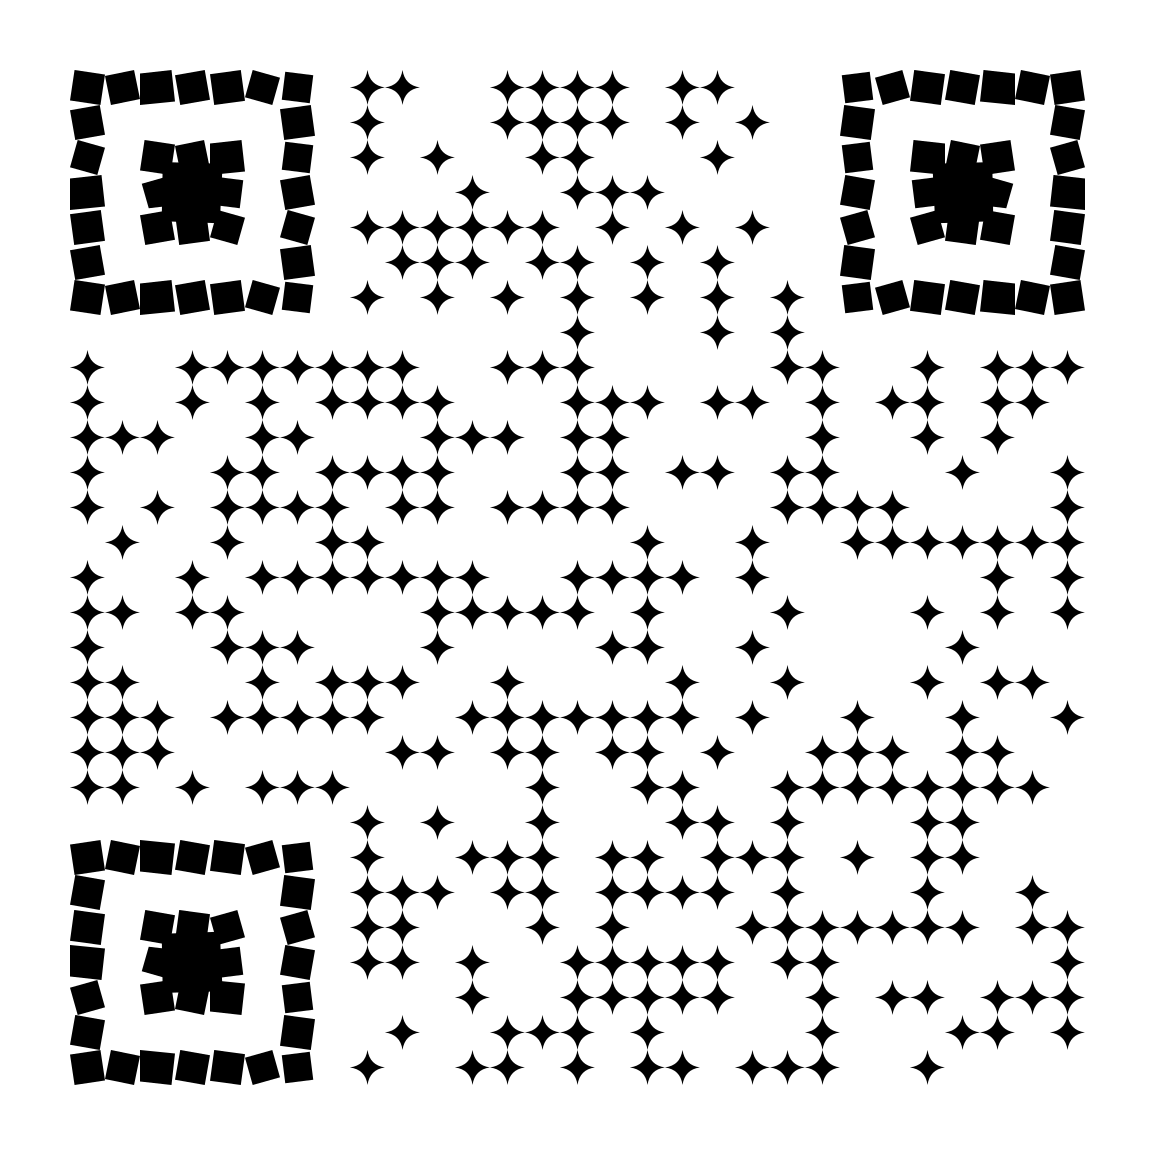
\includegraphics[width=7cm]{./img/qr-code-feedback.png}

\url{https://forms.gle/AdWrxLSsYz2nCf1j7}

\end{center}

\end{document}
